% Options for packages loaded elsewhere
\PassOptionsToPackage{unicode}{hyperref}
\PassOptionsToPackage{hyphens}{url}
%
\documentclass[
  ignorenonframetext,
  aspectratio=169]{beamer}
\usepackage{pgfpages}
\setbeamertemplate{caption}[numbered]
\setbeamertemplate{caption label separator}{: }
\setbeamercolor{caption name}{fg=normal text.fg}
\beamertemplatenavigationsymbolsempty
% Prevent slide breaks in the middle of a paragraph
\widowpenalties 1 10000
\raggedbottom
\setbeamertemplate{part page}{
  \centering
  \begin{beamercolorbox}[sep=16pt,center]{part title}
    \usebeamerfont{part title}\insertpart\par
  \end{beamercolorbox}
}
\setbeamertemplate{section page}{
  \centering
  \begin{beamercolorbox}[sep=12pt,center]{part title}
    \usebeamerfont{section title}\insertsection\par
  \end{beamercolorbox}
}
\setbeamertemplate{subsection page}{
  \centering
  \begin{beamercolorbox}[sep=8pt,center]{part title}
    \usebeamerfont{subsection title}\insertsubsection\par
  \end{beamercolorbox}
}
\AtBeginPart{
  \frame{\partpage}
}
\AtBeginSection{
  \ifbibliography
  \else
    \frame{\sectionpage}
  \fi
}
\AtBeginSubsection{
  \frame{\subsectionpage}
}
\usepackage{amsmath,amssymb}
\usepackage{lmodern}
\usepackage{iftex}
\ifPDFTeX
  \usepackage[T1]{fontenc}
  \usepackage[utf8]{inputenc}
  \usepackage{textcomp} % provide euro and other symbols
\else % if luatex or xetex
  \usepackage{unicode-math}
  \defaultfontfeatures{Scale=MatchLowercase}
  \defaultfontfeatures[\rmfamily]{Ligatures=TeX,Scale=1}
\fi
\usetheme[]{metropolis}
% Use upquote if available, for straight quotes in verbatim environments
\IfFileExists{upquote.sty}{\usepackage{upquote}}{}
\IfFileExists{microtype.sty}{% use microtype if available
  \usepackage[]{microtype}
  \UseMicrotypeSet[protrusion]{basicmath} % disable protrusion for tt fonts
}{}
\makeatletter
\@ifundefined{KOMAClassName}{% if non-KOMA class
  \IfFileExists{parskip.sty}{%
    \usepackage{parskip}
  }{% else
    \setlength{\parindent}{0pt}
    \setlength{\parskip}{6pt plus 2pt minus 1pt}}
}{% if KOMA class
  \KOMAoptions{parskip=half}}
\makeatother
\usepackage{xcolor}
\newif\ifbibliography
\usepackage{graphicx}
\makeatletter
\def\maxwidth{\ifdim\Gin@nat@width>\linewidth\linewidth\else\Gin@nat@width\fi}
\def\maxheight{\ifdim\Gin@nat@height>\textheight\textheight\else\Gin@nat@height\fi}
\makeatother
% Scale images if necessary, so that they will not overflow the page
% margins by default, and it is still possible to overwrite the defaults
% using explicit options in \includegraphics[width, height, ...]{}
\setkeys{Gin}{width=\maxwidth,height=\maxheight,keepaspectratio}
% Set default figure placement to htbp
\makeatletter
\def\fps@figure{htbp}
\makeatother
\setlength{\emergencystretch}{3em} % prevent overfull lines
\providecommand{\tightlist}{%
  \setlength{\itemsep}{0pt}\setlength{\parskip}{0pt}}
\setcounter{secnumdepth}{-\maxdimen} % remove section numbering
\newlength{\cslhangindent}
\setlength{\cslhangindent}{1.5em}
\newlength{\csllabelwidth}
\setlength{\csllabelwidth}{3em}
\newlength{\cslentryspacingunit} % times entry-spacing
\setlength{\cslentryspacingunit}{\parskip}
\newenvironment{CSLReferences}[2] % #1 hanging-ident, #2 entry spacing
 {% don't indent paragraphs
  \setlength{\parindent}{0pt}
  % turn on hanging indent if param 1 is 1
  \ifodd #1
  \let\oldpar\par
  \def\par{\hangindent=\cslhangindent\oldpar}
  \fi
  % set entry spacing
  \setlength{\parskip}{#2\cslentryspacingunit}
 }%
 {}
\usepackage{calc}
\newcommand{\CSLBlock}[1]{#1\hfill\break}
\newcommand{\CSLLeftMargin}[1]{\parbox[t]{\csllabelwidth}{#1}}
\newcommand{\CSLRightInline}[1]{\parbox[t]{\linewidth - \csllabelwidth}{#1}\break}
\newcommand{\CSLIndent}[1]{\hspace{\cslhangindent}#1}
\ifLuaTeX
\usepackage[bidi=basic]{babel}
\else
\usepackage[bidi=default]{babel}
\fi
\babelprovide[main,import]{brazilian}
% get rid of language-specific shorthands (see #6817):
\let\LanguageShortHands\languageshorthands
\def\languageshorthands#1{}
\setbeameroption{show notes}
\setbeamerfont{note page}{size=\footnotesize}
\hypersetup{colorlinks,citecolor=orange,filecolor=red,linkcolor=brown,urlcolor=blue}
\pgfdeclareimage[height=2cm]{qrcode}{qrcode.png}
\titlegraphic{\pgfuseimage{qrcode}}
\usepackage{phonrule}
% https://tex.stackexchange.com/questions/625478/beamer-footnote-in-a-slide-note
\makeatletter
\addtobeamertemplate{note page}{}{
    \begingroup
    \vfill
    \usebeamercolor*[fg]{footnote}%
    \footnoterule%
    \unvbox \beamer@footins%
    \global\setbox\beamer@footins=\box\voidb@x%
    \endgroup  
    \vskip0.2cm
}
\makeatother




\ifLuaTeX
  \usepackage{selnolig}  % disable illegal ligatures
\fi
\IfFileExists{bookmark.sty}{\usepackage{bookmark}}{\usepackage{hyperref}}
\IfFileExists{xurl.sty}{\usepackage{xurl}}{} % add URL line breaks if available
\urlstyle{same} % disable monospaced font for URLs
\hypersetup{
  pdftitle={Linguistíca Quantitativa},
  pdfauthor={Leonardo Araujo},
  pdflang={pt-BR},
  hidelinks,
  pdfcreator={LaTeX via pandoc}}

\title{Linguistíca Quantitativa}
\author{Leonardo Araujo}
\date{23 de Novembro de 2022}

\begin{document}
\frame{\titlepage}

\hypertarget{linguuxedstica-quantitativa-enquanto-ciuxeancia}{%
\section{Linguística Quantitativa enquanto
ciência}\label{linguuxedstica-quantitativa-enquanto-ciuxeancia}}

\begin{frame}{Leis}
\protect\hypertarget{leis}{}
\begin{itemize}
\tightlist
\item
  Lei científica
\end{itemize}

~

\begin{quote}
Uma lei científica é um princípio básico, generalização ou regra que se
mantém universalmente verdadeira sob condições particulares
(\protect\hyperlink{ref-mccomas2014}{McComas 2014}).
\end{quote}

\note{Uma lei, em ciência, é uma hipótese sistematicamente conectada a
outras hipóteses em um campo do conhecimento e, ao mesmo tempo,
corroborada por dados empíricos. Uma lei é dita universal quando é
valida a todo tempo, em qualquer lugar e para todos objetos sob seu
escopo.}
\end{frame}

\begin{frame}{Exemplos}
\protect\hypertarget{exemplos}{}
\begin{figure}
\centering
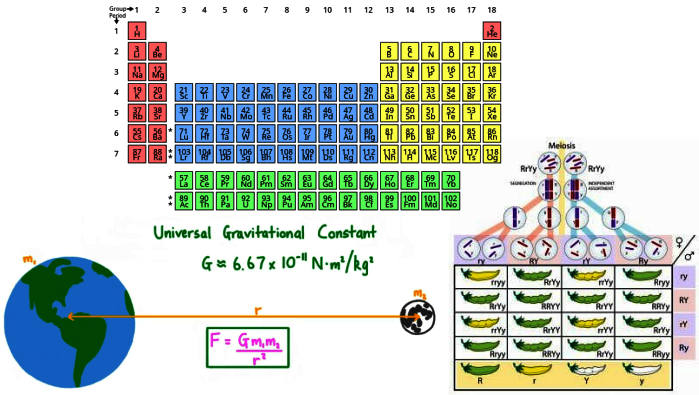
\includegraphics[width=0.7\textwidth,height=\textheight]{laws-grav-per-men.png}
\caption{Lei da gravidade
(\url{https://www.nagwa.com/en/videos/346134549365/}). Lei periódica
(\url{https://en.wikipedia.org/wiki/Periodic_table}). Lei de Mendel
(\url{https://biologydictionary.net/mendels-law-of-heredity/}).}
\end{figure}

\note{A \textbf{lei da gravidade} prediz a força de atração entre copos
com base em suas massas e distância entre eles. Entretanto, não explica
o motivo da existência de tal atração ou busca explicar o motivo pelo
qual tal comportamento é descrito pela equação
\(F = G\frac{m_1 m_2}{r^2}\).

A \textbf{lei periódica} estabelece que certas propriedades físicas e
químicas dos elementos serão recorrentes de maneira sistemática e
previsível quando os elementos são ordenados de forma crescente de seus
número atômico. As principais propriedades em que observamos uma
tendência devido à lei da periodicidade são: raio atômico, raio iônico,
energia de ionização, eletronegatividade e eletroafinidade.

As \textbf{leis de Mendel} (ou leis da herança) são as três leis a
seguir: 1) lei da dominância (quando pais com traços puros e
contrastantes são cruzados, apenas uma forma de traço aparece na próxima
geração; assim, os descendentes híbridos exibirão apenas a
característica dominante no fenótipo); 2) lei da segregação (uma única
característica associada a um único gene é herdada); e 3) lei da
variação independente (os alelos de dois (ou mais) genes diferentes são
distribuídos para os gametas independentemente um do outro).}
\end{frame}

\begin{frame}{Teoria}
\protect\hypertarget{teoria}{}
\begin{itemize}
\tightlist
\item
  Teoria: um sistema de leis

  \begin{itemize}
  \tightlist
  \item
    teorias axiomáticas
  \item
    teorias empíricas
  \end{itemize}
\end{itemize}

\note{Compreendemos ciência como um esforço sistemático de construir e
organizar conhecimento na forma de explicações e predições testáveis
sobre o universo.

Um sistema de leis é chamado de Teoria. A construção de uma teoria é
principal objetivo de pesquisas científicas.

~

A filosofia da ciência distingue dois tipos de teorias: 1) as teorias
axiomáticas da lógica e matemática (utiliza um sistema axiomático para
construir verdades analíticas); 2) as teorias empíricas da ciência
factual (faz afirmações sobre partes do mundo; a veracidade dependerá da
correção interna e correspondência com fatos da realidade; teorias
empíricas devem também ter um núcleo axiomático).}
\end{frame}

\begin{frame}{Linguistíca Quantitativa}
\protect\hypertarget{linguistuxedca-quantitativa}{}
\begin{itemize}
\tightlist
\item
  Linguística formal - matemática qualitativa (álgebra, teoria de
  conjuntos e lógica)
\end{itemize}

\onslide<2->{
\begin{footnotesize}
Exemplo para o português brasileiro:
\begin{center}
\phonb{\phonfeat{+silábico \\ +alto \\ -arredondado}
}{∅}{\#}{\phonfeat{+consonantal \\ +contínuo \\ +coronal}\phonfeat{+consonantal}}
\end{center}
A vogal [i] pode ser apagada em início de palavra quando seguida de uma sibilante e outra consoante. Por
exemplo: esperar, estragar, espelho, estante, etc.
\end{footnotesize}
}

\begin{itemize}
\tightlist
\item
  Linguística quantitativa (LQ) - propriedades quantitativas
  (quantidades, probabilidades e tendências)
\end{itemize}

\note{Linguística formal utiliza-se de princípios da matemática
qualitativa (álgebra, teoria de conjuntos e lógica) para modelar
propriedades estruturais da linguagem.

~

A linguística quantitativa (LQ) estuda as diversas propriedades
quantitativas, essenciais para a descrição e compreensão dos sistemas
linguísticos. A LQ lida com quantidades, probabilidades e tendências,
analisando comprimento, frequência, distância, grau de polissemia,
idade, etc. As propriedades de elementos linguísticos e suas
inter-relações são formuladas matematicamente, estabelecendo leis
estocásticas (ou seja, não capturam casos singulares, mas predizem
eventos e condições gerais). A abordagem quantitativa permite uma
descrição mais adequada da realidade, permitindo a distinção em diversos
níveis ao invés de uma distinção extrema em apenas dois extremos
(sim/não).}
\end{frame}

\begin{frame}{Surgimento da linguística quantitativa}
\protect\hypertarget{surgimento-da-linguuxedstica-quantitativa}{}
\begin{itemize}
\tightlist
\item
  George Kingley Zipf - a lei de Zipf

  \begin{itemize}
  \tightlist
  \item
    relação entre ordem (rank) e frequência -- princípio de
    auto-organização e economicidade
  \item
    ``The Psycho-Biology of Language. An Introduction to Dynamic
    Philology'' (1935)
  \item
    ``Human Behavior and the Principle of Least Effort'' (1949)
  \end{itemize}
\end{itemize}

\note{Embora diversos trabalho abordasse a quantificação de unidades
linguísticas, antes mesmo no século XIX, George Kingley Zipf é
considerado o pai da linguística quantitativa por ter sistematicamente
investigado e criado um modelo teórico para explicar suas observações e
propor uma formulação matemática.

~

Zipf propôs as ideias de

\begin{itemize}
\tightlist
\item
  princípio do esforço mínimo (esforço mínimo individual e esforço
  mínimo coletivo)
\item
  forças de unificação e diversificação
\end{itemize}

Para o falante, o princípio da economia busca uma maior unificação e
simplificação (o que dificulta a tarefa do ouvinte). Para o ouvinte, o
princípio da economia busca diversificação (o que simplifica sua tarefa
de decodificação da mensagem, mas dificulta a tarefa do falante).}
\end{frame}

\hypertarget{leis-da-linguuxedstica-quantitativa}{%
\section{Leis da Linguística
Quantitativa}\label{leis-da-linguuxedstica-quantitativa}}

\begin{frame}{Lei de Zipf}
\protect\hypertarget{lei-de-zipf}{}
Zipf (\protect\hyperlink{ref-zipf1949}{1949}) - Ulysses de James Joyce -
260.430 palavras (29.899 palavras diferentes).

Relação entre rank e frequência de ocorrência.

\begin{equation} r \times f = C \label{eq:zipflaw}\end{equation}

Ao visualizar tal relação em um gráfico log-log, esperamos ver uma reta
com inclinação -1.

\begin{align}
       f &= \frac{C}{r} \\
  \log f &= -\log r + \log C
  \end{align}

\note{Zipf analisou o livro Ulysses de James Joyce. O texto possui
260.430 palavras, sendo 29.899 palavras diferentes.

\begin{itemize}
\item
  palavras foram consideradas diferentes se diferem-se foneticamente na
  forma flexionada que ocorrem no texto (desta forma, give, gives, gave,
  given, giving, giver e gift representam sete palavras diferentes e não
  uma única palavras com sete formas diferentes).
\item
  Zipf observou uma correlação entre o número de diferentes palavras e
  sua frequência de uso, aproximando-se à equação de uma hipérbole
  equilátera\footnote{Dizemos que uma hipérbole é equilátera se o comprimento do eixo focal é igual ao comprimento do eixo não-focal.}
  \(y=1/x\) (lei de Zipf inversa).
\end{itemize}}
\end{frame}

\begin{frame}
\begin{figure}
\centering
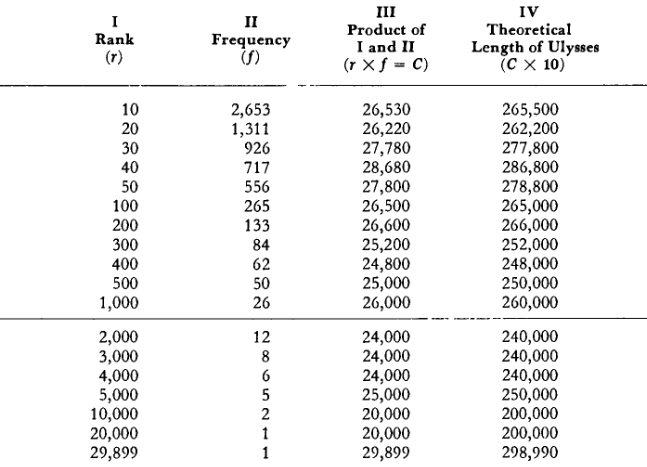
\includegraphics[width=0.65\textwidth,height=\textheight]{zipf-tab2-1-ulysses.png}
\caption{Tabela com alguns exemplos de rank e frequência de ocorrência
de palavras em Ulysses (\protect\hyperlink{ref-zipf1949}{Zipf 1949}).}
\end{figure}
\end{frame}

\begin{frame}
\begin{figure}
\centering
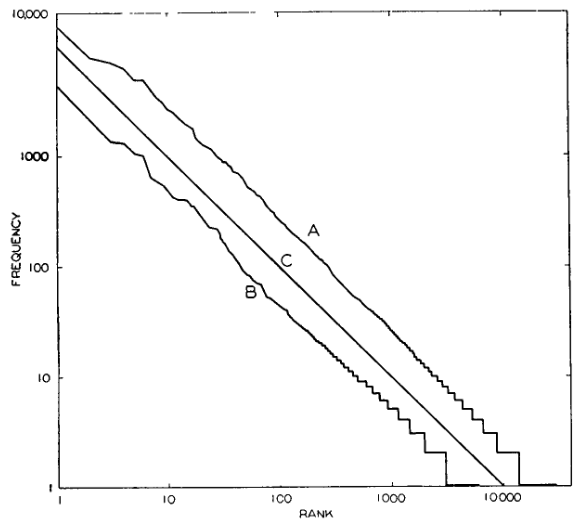
\includegraphics[width=0.5\textwidth,height=\textheight]{zipf-fig2-1-ulysses.png}
\caption{Distribuição rank-frequência para palavras no inglês. (A) dados
de James Joyce; (B) dados de Eldridge (43.989 palavras de jornais, sendo
6.002 palavras diferentes); (C) curva ideal com inclinação igual a 1
(\protect\hyperlink{ref-zipf1949}{Zipf 1949}).}
\end{figure}

\note{Os degraus ao final representam palavras com baixa frequência de
ocorrência. Como apenas é possível observarmos as palavras um numero
inteiro de vez, o valor da relação dada na equação
\protect\hyperlink{eq:zipflaw}{1} é arredondado para o inteiro mais
próximo.

O último degrau representa 16.432 palavras que ocorreram uma única vez
em todo o texto (hápax legómenon). O degrau anterior representa 4.776
palavras que ocorreram duas vezes (dis legomenon) e o anterior
representa 2.194 palavras que ocorreram três vezes (tris legomenon).}
\end{frame}

\begin{frame}
\begin{figure}
\centering
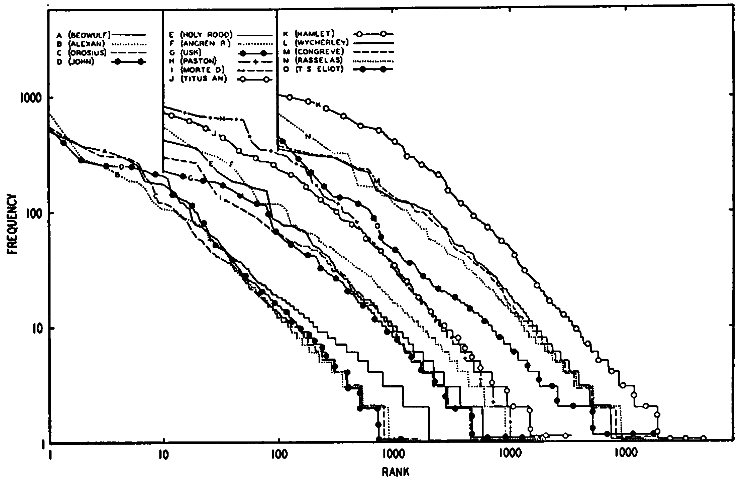
\includegraphics[width=0.7\textwidth,height=\textheight]{zipf-fig3-14.png}
\caption{De Beowulf a T.S. Eliot. Distribuição rank-frequência de
palavras em 15 escritores da língua inglesa, do inglês antigo ao atual.
Os gráficos estão deslocados na abscissa para melhor visualização.}
\end{figure}
\end{frame}

\begin{frame}{Lei de Zipf}
\protect\hypertarget{lei-de-zipf-1}{}
A \(r\)-ésima palavra mais frequente possui frequência de ocorrência
\(f(r)\) que varia da seguinte forma com \(r\): \[
f \propto \frac{1}{r^{\alpha}}
\] onde temos \(\alpha \approx 1\)
(\protect\hyperlink{ref-zipf1935}{Zipf 1935},
\protect\hyperlink{ref-zipf1949}{1949}).

\note{Outros trabalhos mostram que o valor do expoente \(\alpha\) está
entre 0.6 e 1.5 para o inglês falado
(\protect\hyperlink{ref-Bian2016}{Bian et al. 2016};
\protect\hyperlink{ref-Baixeries2013}{Baixeries, Elvevåg, e
Ferrer-i-Cancho 2013}), entre 0.765 e 1.357 para traduções da bíblia em
diversas línguas (\protect\hyperlink{ref-mehri2017}{Mehri e Jamaati
2017}).}
\end{frame}

\begin{frame}
\begin{figure}
\centering
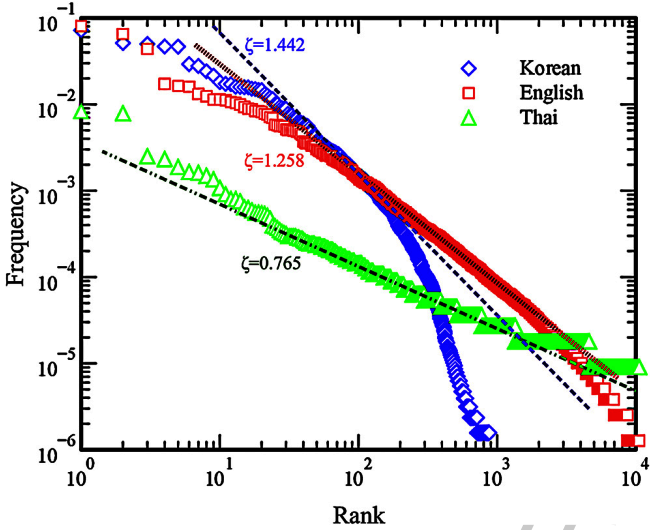
\includegraphics[width=0.6\textwidth,height=\textheight]{mehri-fig2.png}
\caption{Gráfico Zipf para tradução da bíblia no coreano, inglês e
tailandês (\protect\hyperlink{ref-mehri2017}{Mehri e Jamaati 2017}).}
\end{figure}

\note{Em seu trabalho, Mehri e Jamaati
(\protect\hyperlink{ref-mehri2017}{2017}) faz o ajuste da distribuição
de Zipf para a tradução da bíblia em 100 línguas diferentes. Mehri e
Jamaati (\protect\hyperlink{ref-mehri2017}{2017}) enfatiza que
estruturas sintáticas distintas levam a expoentes de Zipf diferentes e
analisam o comportamento do coeficiente de Zipf em diferentes famílias
linguísticas.

Inglês e Coreano possuem coeficiente de Zipf próximos, enquanto o
tailandês possui coeficiente bem diferente, o que pode ser explicado
pela sua estrutura gramatical distinta. A lei de Zipf não é compatível
com dados empíricos de palavras de tipo raro. Benoit Mandelbrot
(\protect\hyperlink{ref-mandelbrot1966information}{1966}) generalizou a
lei de Zipf para superar tal limitação.}
\end{frame}

\begin{frame}
Esta relação de potência é também observada em outros diferentes
fenômenos, tais como:

\begin{itemize}
\tightlist
\item
  magnitude de terremotos (\protect\hyperlink{ref-suzuki2005}{Abe e
  Suzuki 2005});
\item
  população de cidades (\protect\hyperlink{ref-gabaix1999}{Gabaix
  1999});
\item
  variações de preços (\protect\hyperlink{ref-mandelbrot1963}{Benoît
  Mandelbrot 1963});
\item
  distribuição do passivo total de empresas falidas
  (\protect\hyperlink{ref-fujiwara2004}{Fujiwara 2004});
\item
  expressão gênica (\protect\hyperlink{ref-furusawa}{Furusawa e Kaneko
  2003});
\item
  sistemas dinâmicos caóticos
  (\protect\hyperlink{ref-nicolis1989}{Nicolis, Nicolis, e Nicolis
  1989});
\item
  magnitude de avalanches (\protect\hyperlink{ref-perbak}{Bak 1996});
\item
  tráfegos de dados na Internet
  (\protect\hyperlink{ref-crovella96}{Crovella e Bestavros 1996});
\item
  requisições de páginas web
  (\protect\hyperlink{ref-huberman2002}{Adamic e Huberman 2002});
\item
  número de citações de artigos científicos
  (\protect\hyperlink{ref-derek1965}{Solla Price 1965});
\item
  tamanho das famílias linguísticas
  (\protect\hyperlink{ref-wichmann2005}{Wichmann 2005});
\item
  tiragem de livros e discos (\protect\hyperlink{ref-kohli}{Kohli e Sah
  2003}; \protect\hyperlink{ref-cox}{Cox, Felton, e Chung 1995});
\end{itemize}

e muitos outros.
\end{frame}

\begin{frame}
\begin{figure}
\centering
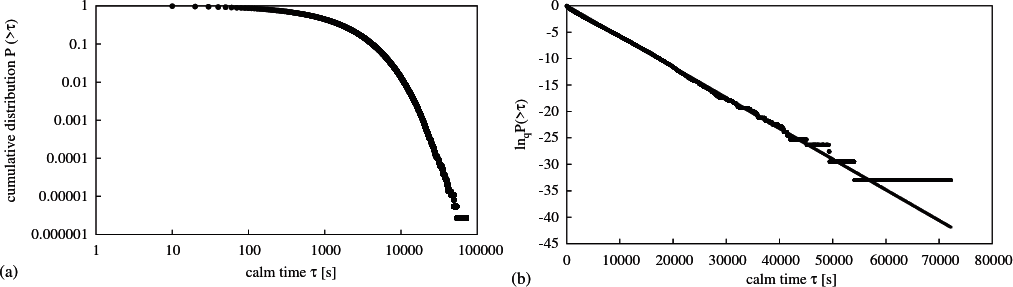
\includegraphics[width=1\textwidth,height=\textheight]{abe-earthquakes.png}
\caption{Distribuição cumulativa dos tempos calmos (entre terremotos) na
California (\protect\hyperlink{ref-suzuki2005}{Abe e Suzuki 2005}).}
\end{figure}
\end{frame}

\begin{frame}
\begin{figure}
\centering
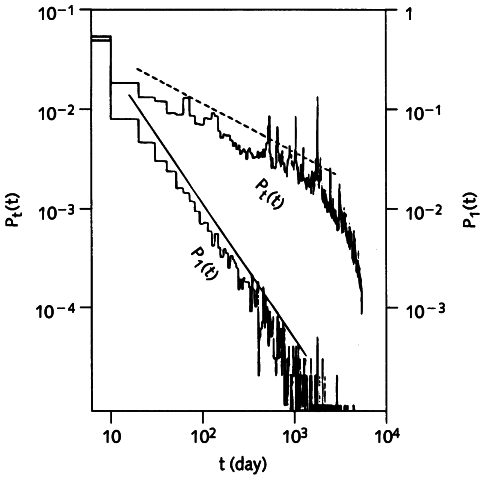
\includegraphics[width=0.5\textwidth,height=\textheight]{bak-earthquakes.png}
\caption{Distribuição do tempo entre terremotos (tempo de primeiro
retorno e todos) (\protect\hyperlink{ref-perbak}{Bak 1996};
\protect\hyperlink{ref-ito1990earthquakes}{Ito e Matsuzaki 1990}).}
\end{figure}
\end{frame}

\begin{frame}
\begin{figure}
\centering
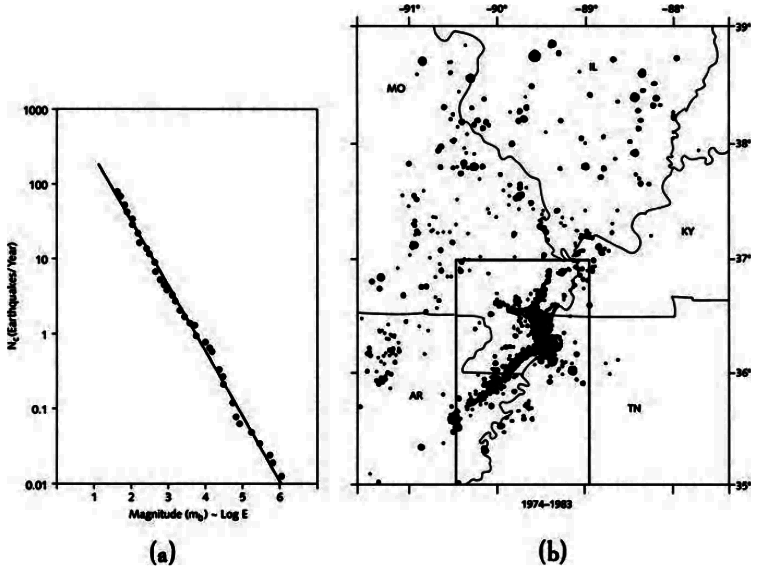
\includegraphics[width=0.5\textwidth,height=\textheight]{bak-earthquakes2.png}
\caption{Distribuição da magnitude de terremotos. Os pontos representam
o número de terremotos \(N_c\) com magnitude maior que uma determinada
magnitude \(m\). A figura (b) apresenta a localização dos terremotos em
Nova Madrid (Missouri) nos anos de 1974 a 1983. O tamanho dos pontos
representa a magnitude dos terremotos
(\protect\hyperlink{ref-perbak}{Bak 1996}).}
\end{figure}
\end{frame}

\begin{frame}
\begin{figure}
\centering
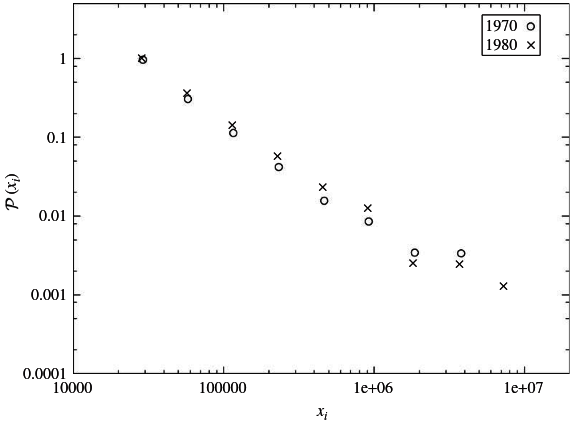
\includegraphics[width=0.6\textwidth,height=\textheight]{ribeiro-pop-cidades.png}
\caption{Distribuição cumulativa \(P(x_i)\) das cidades brasileiras com
população \(x_i\) (\protect\hyperlink{ref-moura2006zipf}{Moura Jr e
Ribeiro 2006}).}
\end{figure}
\end{frame}

\begin{frame}
\begin{figure}
\centering
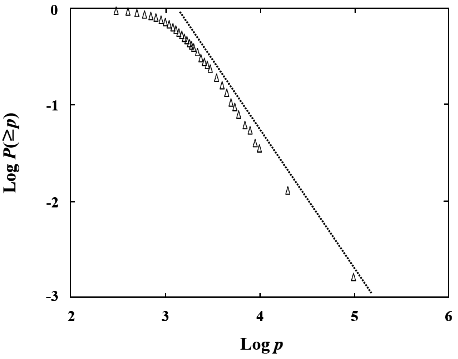
\includegraphics[width=0.6\textwidth,height=\textheight]{choi-koren-stock.png}
\caption{Distribuição cumulativa dos preços de ações negocinadas no
KOSDAQ (Korean Securities Dealers Automated Quotations)
(\protect\hyperlink{ref-choi2005}{Choi et al. 2005}).}
\end{figure}
\end{frame}

\begin{frame}
\begin{figure}
\centering
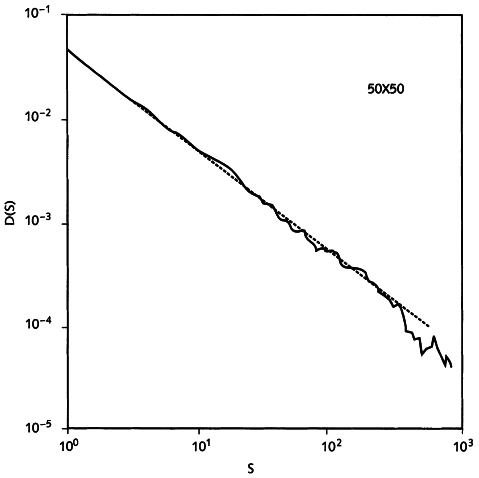
\includegraphics[width=0.55\textwidth,height=\textheight]{bak-avalanches.png}
\caption{Distribuição de avalanches (\(s\) representa o tamanho das
avalanches) (\protect\hyperlink{ref-perbak}{Bak 1996}).}
\end{figure}
\end{frame}

\begin{frame}
\begin{figure}
\centering
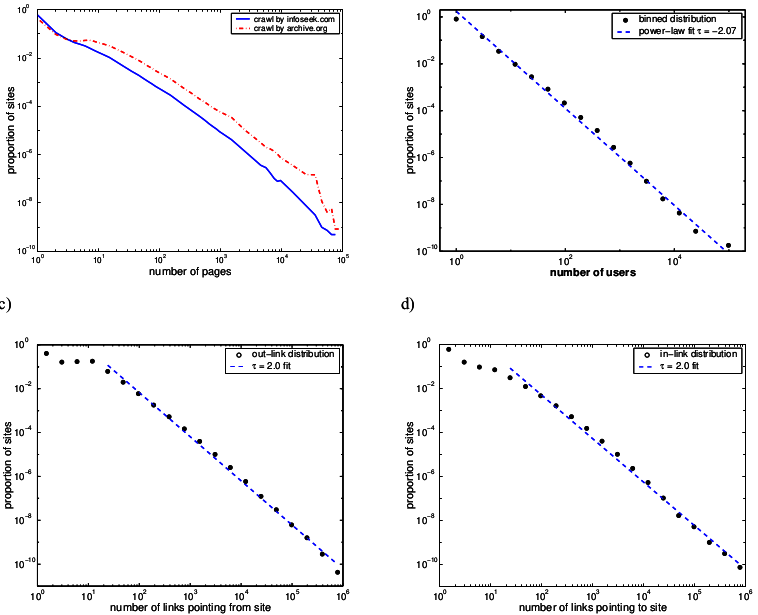
\includegraphics[width=0.6\textwidth,height=\textheight]{adamic-sites.png}
\caption{Distribuição de lei de potência para o número de a) páginas, b)
visitantes, c) links externos e d) links internos de um site (medidas de
1997) (\protect\hyperlink{ref-huberman2002}{Adamic e Huberman 2002}).}
\end{figure}
\end{frame}

\begin{frame}
\begin{figure}
\centering
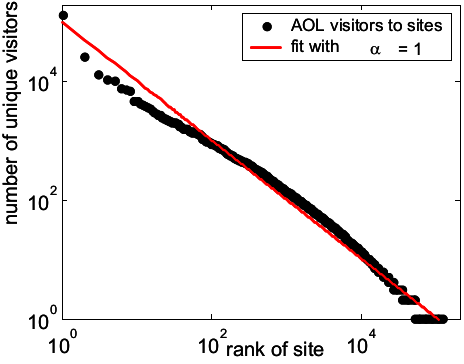
\includegraphics[width=0.5\textwidth,height=\textheight]{adamic-visitors.png}
\caption{Sites ordenados pelo número de visitantes AOL únicos recebidos
em 01/12/1997 (\protect\hyperlink{ref-huberman2002}{Adamic e Huberman
2002}).}
\end{figure}
\end{frame}

\begin{frame}
\begin{figure}
\centering
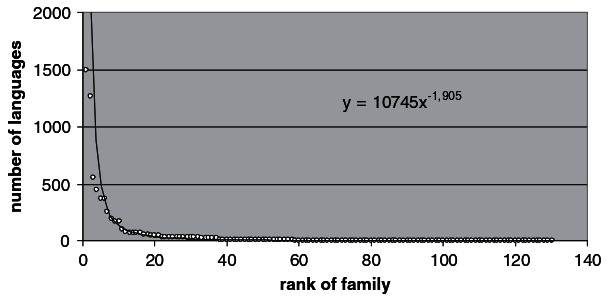
\includegraphics[width=0.8\textwidth,height=\textheight]{wichmann2005_familysize.png}
\caption{Tamanho das famílias linguísticas, segundo Grimes
(\protect\hyperlink{ref-grimes2000}{2000};
\protect\hyperlink{ref-wichmann2005}{Wichmann 2005}).}
\end{figure}
\end{frame}

\begin{frame}{Generalização proposta por Mandelbrot}
\protect\hypertarget{generalizauxe7uxe3o-proposta-por-mandelbrot}{}
Benoît Mandelbrot (\protect\hyperlink{ref-mandelbrot1963}{1963}) propôs
um deslocamento para levar em consideração o achatamento observado na
região do baixo ranque

\[
f \propto \frac{1}{(r + \beta)^{\alpha}}
\]

em que \(\alpha \approx 1\) e \(\beta \approx 2.7\)
(\protect\hyperlink{ref-zipf1935}{Zipf 1935},
\protect\hyperlink{ref-zipf1949}{1949};
\protect\hyperlink{ref-mandelbrot1963}{Benoît Mandelbrot 1963}).
\end{frame}

\begin{frame}[allowframebreaks]{Por que as línguas seguem a lei de
Zipf?}
\protect\hypertarget{por-que-as-luxednguas-seguem-a-lei-de-zipf}{}
Algumas possíveis explicações:

\begin{itemize}
\tightlist
\item
  processos aleatórios concatenativos
  (\protect\hyperlink{ref-conrad2004power}{Conrad e Mitzenmacher 2004};
  \protect\hyperlink{ref-li1992random}{Li 1992};
  \protect\hyperlink{ref-miller1957some}{Miller 1957})
\item
  mistura de distribuições exponenciais
  (\protect\hyperlink{ref-farmer2008power}{Farmer e Geanakoplos 2008})
\item
  invariância à escala (\protect\hyperlink{ref-chater1999scale}{Chater e
  Brown 1999})
\item
  otimização (com restrição) da entropia
  (\protect\hyperlink{ref-mandelbrot1953}{B. B. Mandelbrot 1953})
\item
  otimização da informação de Fisher
  (\protect\hyperlink{ref-hernando2009zipf}{Hernando et al. 2009})
\item
  invariância das leis de potência sob agregação
  (\protect\hyperlink{ref-farmer2008power}{Farmer e Geanakoplos 2008})
\item
  processos estocásticos multiplicativos
  (\protect\hyperlink{ref-mitzenmacher2004brief}{Mitzenmacher 2004})
\item
  reuso preferencial (\protect\hyperlink{ref-simon1955class}{Simon
  1955}; \protect\hyperlink{ref-yule1944statistical}{Yule 1944})
\item
  descrição simbólica de sistemas complexos de processos estocásticos
  (\protect\hyperlink{ref-corominas2010universality}{Corominas-Murtra e
  Solé 2010})
\item
  passeio aleatório em escalas logarítmicas
  (\protect\hyperlink{ref-kawamura2002universality}{Kawamura e Hatano
  2002})
\item
  organização semântica
  (\protect\hyperlink{ref-guiraud1968semic}{Guiraud 1968};
  \protect\hyperlink{ref-manin2008zipf}{Manin 2008})
\item
  otimização da comunicação (\protect\hyperlink{ref-cancho2003}{Cancho e
  Solé 2003}; \protect\hyperlink{ref-cancho2005decoding}{Cancho 2005};
  \protect\hyperlink{ref-cancho2005hidden}{R. Ferrer-i-Cancho 2005};
  \protect\hyperlink{ref-mandelbrot1963}{Benoît Mandelbrot 1963};
  \protect\hyperlink{ref-salge2015zipf}{Salge et al. 2015};
  \protect\hyperlink{ref-zipf1935}{Zipf 1935},
  \protect\hyperlink{ref-zipf1949}{1949})
\item
  divisão aleatória de elementos em grupos
  (\protect\hyperlink{ref-baek2011zipf}{Baek, Bernhardsson, e Minnhagen
  2011})
\item
  aproximação de primeira e segunda ordem de distribuições comuns
  (normal, por exemplo) (\protect\hyperlink{ref-baek2011zipf}{Baek,
  Bernhardsson, e Minnhagen 2011})
\item
  busca otimizada em memória
  (\protect\hyperlink{ref-parker1956theory}{Parker-Rhodes e Joyce 1956})
\item
  etc.
\end{itemize}

\note{É razoável esperar que as palavras não sejam igualmente
distribuídas, entretanto, dado que as palavras tem frequências
distintas, por qual razão seguiriam uma regra matemática particular?
Sobretudo, por que seguiriam uma regra que não leva em consideração o
significado ou função sintática das palavras?}
\end{frame}

\begin{frame}{Invariância à escala}
\protect\hypertarget{invariuxe2ncia-uxe0-escala}{}
\begin{figure}
\centering
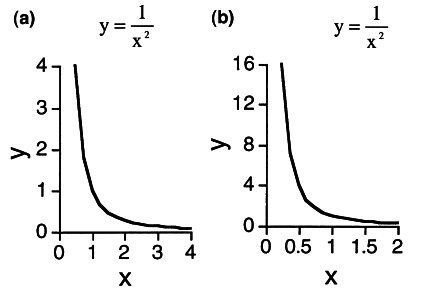
\includegraphics[width=0.5\textwidth,height=\textheight]{chater-invariancia-escala.png}
\caption{Conceito de invariância à escala. A mesma função é apresentada
em diferentes escalas (\protect\hyperlink{ref-chater1999scale}{Chater e
Brown 1999}).}
\end{figure}

\note{Para Chater e Brown
(\protect\hyperlink{ref-chater1999scale}{1999}), o sistema
perceptual-motor reflerem e preservam a características de invariância a
escala presentes em vários aspectos ambientais. Isto permite o
surgimento de diversas leis da psicologia governando perceção e ação em
vários domínios e espécies (exemplos: lei de Weber-Fechner, lei de
Stevens, lei de Fitts e lei de Piéron).}
\end{frame}

\begin{frame}{Lei de Zipf evitando sinonímia excessiva}
\protect\hypertarget{lei-de-zipf-evitando-sinonuxedmia-excessiva}{}
\begin{figure}
\centering
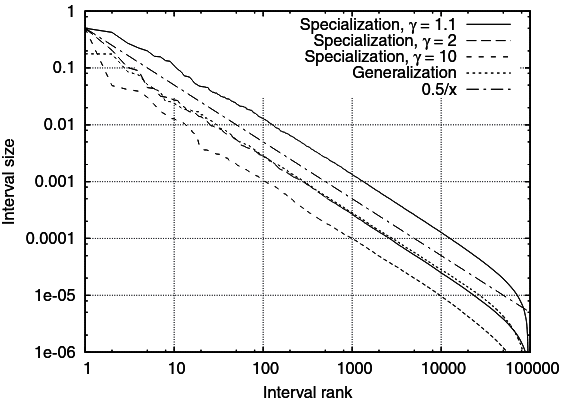
\includegraphics[width=0.6\textwidth,height=\textheight]{manin2008-intervals.png}
\caption{Lei de Zipf gerada por modelos de especialização e
generalização. O parâmetro \(\gamma\) determina o quanto duas palavras
podem diferir em extensão e ainda competir entre elas
(\protect\hyperlink{ref-manin2008zipf}{Manin 2008}).}
\end{figure}

\note{Manin (\protect\hyperlink{ref-manin2008zipf}{2008}) sugere que a
lei de Zipf é resultante da organização hierárquica dos significados de
palavras no espaço semântico. Manin
(\protect\hyperlink{ref-manin2008zipf}{2008}) parte da proposta de
matriz semântica de Guiraud
(\protect\hyperlink{ref-guiraud1968semic}{1968}) em que o significado de
uma palavra é representado pela superposição de significados
elementares. Manin (\protect\hyperlink{ref-manin2008zipf}{2008}) propõe
um modelo numérico em que o significado de palavras é associado a
intervalos numéricos e está sujeito ao processo de generalização e
especialização, sendo regido por regras simples. Manin
(\protect\hyperlink{ref-manin2008zipf}{2008}) mostra que este modelo
simples leva à distribuição de Zipf.

Os significados de palavras são associados a subintervalos do intervalo
\(S=[0,1]\){]}. \textbf{Modelo de generalização}: Se não estiverem
congelados, os intervalos vão crescendo paulatinamente por uma
quantidade \(\delta\). Quando surgir uma sobreposição de intervalos, um
deles será escolhido aleatoriamente e será congelado. \textbf{Modelo de
especialização}: Se dois intervalos, \(r_i\) e \(r_j\), se interceptam e
seus comprimentos, \(l_i\) e \(l_j\) satisfazem
\(1/\gamma < l_i/l_j < \gamma\), diminui-se o menor intervalo pelo
tamanho da sobreposição (competição entre os significados de palavras).}
\end{frame}

\begin{frame}{Maximização da informação mútua}
\protect\hypertarget{maximizauxe7uxe3o-da-informauxe7uxe3o-muxfatua}{}
\begin{figure}
\centering
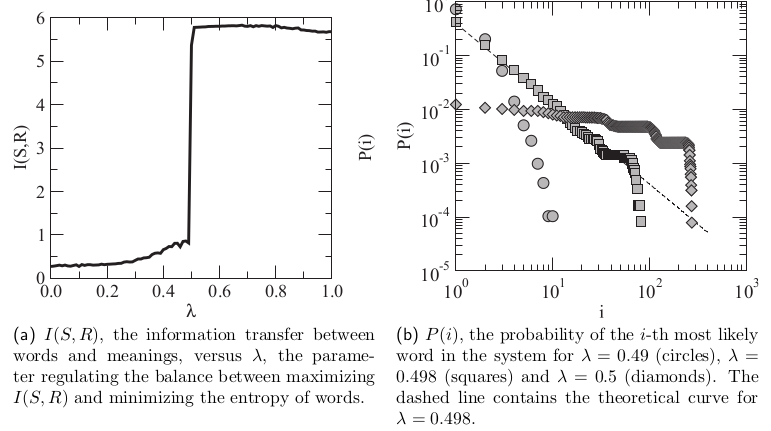
\includegraphics[width=0.7\textwidth,height=\textheight]{cancho-fig1.png}
\caption{Resultado de um modelo computacional onde a probabilidade dos
significados é governada por estruturas internas do sistema de
comunicação. Função minimizada:
\(\Omega(\lambda) = - \lambda I(S,R) + (1-\lambda) H(S)\)
(\protect\hyperlink{ref-cancho2003}{Cancho e Solé 2003};
\protect\hyperlink{ref-cancho2007}{Cancho 2007}).\label{fig-cancho-1}}
\end{figure}

\note{As diversas línguas diferem-se muito, mas todos tem em comum o
fato de serem utilizadas para a comunicação. Um sistema de comunicação
confiável deve maximizar a transferência de informação. Além disto, a
comunicação falada é um processo cognitivo e, portanto, busca-se
economia de energia (para o falante e ouvinte). Cancho e Solé
(\protect\hyperlink{ref-cancho2003}{2003}) utilizam um modelo em que a
comunicação visa à maximização da transferência de informação e a
minimização do custo energético do uso das palavras (entropia).

Cancho e Solé (\protect\hyperlink{ref-cancho2003}{2003});Cancho
(\protect\hyperlink{ref-cancho2007}{2007}) propõe uma função \(\Omega\)
que deve ser minimizada pelo sistema de comunicação. Minimizar esta
função será um balanço entre a maximização da transferência de
comunicação
(\(I(S,R)\))\footnote{Informação mútua entre o sinal e o estímulo.} e
minimizar o custo da comunicação
(\(H(S)\))\footnote{Entropia associada ao sinal.}. A função definida é
\(\Omega(\lambda) = - \lambda I(S,R)+ (1-\lambda) H(S)\), onde o
parâmetro \(\lambda \in [0,1]\) controla o balanço entre a transferência
de informação e o custo. Utilizou-se um algoritmo de Monte Carlo para
realizar a minimização e encontrou-se o valor crítico de
\(\lambda = \lambda^\ast = 1/2 - \epsilon\), onde \(\epsilon\) é um
valor positivo pequeno (\(\epsilon \approx 0.002\) na figura
\ref{fig-cancho-1}). A lei de Zipf ocorre na transição abrupta observada
em \(I(S,R)\), com \(\lambda \approx 1/2\).}
\end{frame}

\begin{frame}[allowframebreaks]{Significado}
\protect\hypertarget{significado}{}
No balanço entre forças de unificação e diversificação esperamos
encontrar palavras que possuam alguns significados.

\begin{itemize}
\tightlist
\item
  \(F_r\): frequência da \(r\)-ésima palavra mais frequente
\item
  \(m_r\): número de significados da \(r\)-ésima palavras mais frequente
\item
  \(f_r\): frequência média de ocorrência dos \(m_r\) significados
\end{itemize}

\[ 
m_r \times f_r = F_r
\]

\begin{itemize}
\tightlist
\item
  forças de unificação: \(\uparrow m_r\), \(\downarrow f_r\)
\item
  forças de diversificação: \(\downarrow m_r\), \(\uparrow f_r\)
\end{itemize}

Uma relação hiperbólica entre as forças leva a

\[
m_r = f_r = \sqrt{F_r}
\]

Em um gráfico log-log da distribuição de frequência dos significados das
palavras, esperamos observar uma reta com inclinação \(-0.5\)
(\protect\hyperlink{ref-zipf1945}{Zipf 1945},
\protect\hyperlink{ref-zipf1949}{1949}).

\note{A princípio, não sabemos qual é o peso dessas duas forças
(unificação e diversificação), porém, pela relação entre o número de
palavras distintas em uma amostra e suas respectivas frequências de
ocorrência, suspeitamos que as forças de unificação e diversificação
estabelecem, em geral, uma relação hiperbólica. Desta forma, resulta-se
em \(m_r\) e \(f_r\) estarem também em uma relação hiperbólica, levado a
obtermos \(m_r = f_r = \sqrt{F_r}\).}
\end{frame}

\begin{frame}
\begin{figure}
\centering
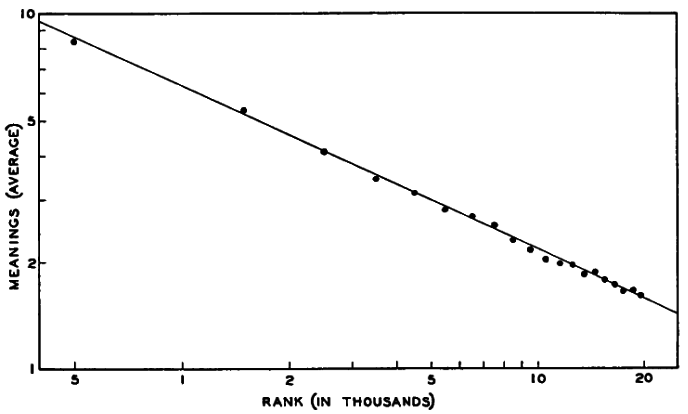
\includegraphics[width=0.8\textwidth,height=\textheight]{zipf-fig2-2.png}
\caption{Distribuição de frequência dos significados das palavras
(\protect\hyperlink{ref-zipf1945}{Zipf 1945},
\protect\hyperlink{ref-zipf1949}{1949}).}
\end{figure}

\note{Zipf (\protect\hyperlink{ref-zipf1949}{1949}) utilizou os dados de
E. L. Thorndike para obter a distribuição de frequência de ocorrência
das palavras (corpus de 10 milhões de palavras) e o Thorndike-Century
Dictionary para obter os \(m\) distintos significados de cada palavra.}
\end{frame}

\begin{frame}{Lei de abreviação/brevidade de Zipf}
\protect\hypertarget{lei-de-abreviauxe7uxe3obrevidade-de-zipf}{}
``a magnitude das palavras apresenta uma relação inversa ao número de
ocorrências'' (\protect\hyperlink{ref-zipf1935}{Zipf 1935})

\begin{figure}
\centering
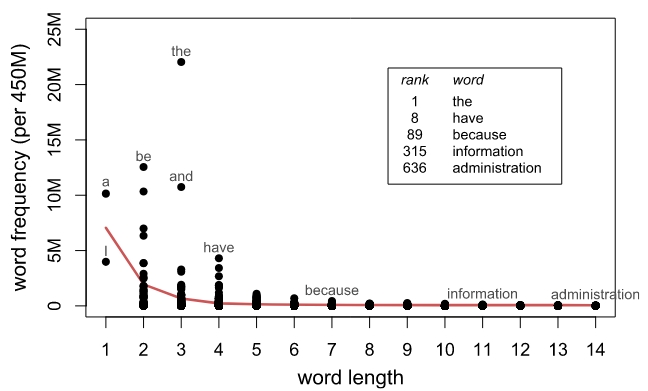
\includegraphics[width=0.65\textwidth,height=\textheight]{kanwal-fig1.png}
\caption{As 1000 palavras mais frequentes no inglês (COCA corpus)
(\protect\hyperlink{ref-kanwal2017}{Kanwal et al. 2017}).}
\end{figure}

\note{Zipf (\protect\hyperlink{ref-zipf1935}{1935}) supôs que tal padrão
seria resultante da relação de compromisso entre uma comunicação sem
erros e um código eficiente (menor esforço). Como as línguas utilizam-se
de um inventário finito de símbolos discretos para formar palavras, o
número de palavras possíveis para um dado comprimento é limitado. Em
palavras curtas, há menos espaço para redundâncias, o que acarreta um
menor potencial de distinguibilidade entre elas. A solução é associar às
palavras curtas os significados mais frequentes e às palavras longas os
significados menos frequentes, abordagem similar ao código de Huffman
(\protect\hyperlink{ref-huffman1952method}{1952}).}
\end{frame}

\begin{frame}
\begin{figure}
\centering
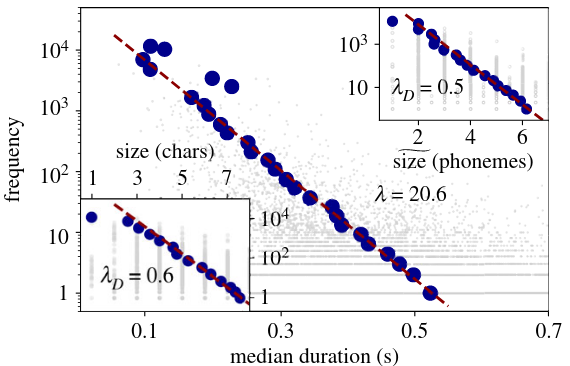
\includegraphics[width=0.7\textwidth,height=\textheight]{brevity.png}
\caption{Lei da brevidade para palavras (duração, número de fonemas e
número de caracteres) (\protect\hyperlink{ref-Torre2019}{Torre et al.
2019}).\label{fig-brevity}}
\end{figure}

\note{Para palavras, Torre et al.
(\protect\hyperlink{ref-Torre2019}{2019}) considera 3 casos para
analisar a lei de brevidade: (1) tendência das palavras mais frequentes
serem constituídas por um menor número de caracteres; (2) tendência das
palavras mais frequentes serem constituídas por um menor número de
fonemas; (3) tendência das palavras mais frequentes serem articuladas
pelos falantes em um menor intervalo de tempo.

Os pontos cinza na figura \ref{fig-brevity} apresentam o espalhamento
das palavras em relação ao tempo mediano de duração (em segundos) e a
frequência de ocorrência das palavras. Os pontos azuis são gerados
através de agrupamento logarítmico nas frequências. O gráfico superior à
direita apresenta o mesmo tipo de relação, porém considerando a mediana
do número de fonemas e o gráfico inferior à esquerda utiliza o numero de
caracteres.

Torre et al. (\protect\hyperlink{ref-Torre2019}{2019}) utilizou o corpus
Buckeye contendo fala de conversação de falantes nativos de inglês,
contendo aproximadamente \(8 \times 10^5\) fonemas, \(3 \times 10^5\)
palavras e \(5 \times 10^4\) grupos
respiratórios\footnote{Grupo respiratório é uma sequência de sons articulados no decorrer de uma única expiração}
(breath-groups).}
\end{frame}

\begin{frame}{Lei da polissemia}
\protect\hypertarget{lei-da-polissemia}{}
\begin{figure}
\centering
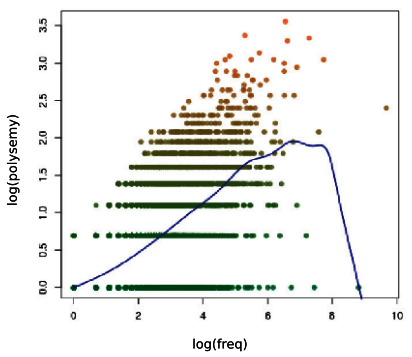
\includegraphics[width=0.4\textwidth,height=\textheight]{polysemy.png}
\caption{Relação entre frequência e polissemia. A cor verde indica a
densidade de pontos (mais escuro, maior densidade). A linha azul é a
regressão não-paramétrica. Dados do corpus SemCor
(\protect\hyperlink{ref-hernandez2016testing}{Hernández-Fernández et al.
2016}).}
\end{figure}

\note{SemCor é um corpus criado pelo Universidade de Princeton, composto
por 352 textos, sendo estes um subconjunto do corpus Brown para o
inglês.}
\end{frame}

\begin{frame}{Leis de polissemia e brevidade de Zipf}
\protect\hypertarget{leis-de-polissemia-e-brevidade-de-zipf}{}
Vários trabalhos analisaram as leis de polissemia e brevidade de Zipf
(\protect\hyperlink{ref-zipf1935}{Zipf 1935},
\protect\hyperlink{ref-zipf1945}{1945};
\protect\hyperlink{ref-hernandez2016testing}{Hernández-Fernández et al.
2016}; \protect\hyperlink{ref-ilgen2007investigation}{Ilgen e Karaoglan
2007}; \protect\hyperlink{ref-cancho2018origins}{Ramon Ferrer-i-Cancho e
Vitevitch 2018}; \protect\hyperlink{ref-kanwal2017}{Kanwal et al. 2017};
\protect\hyperlink{ref-tomaschek2017word}{Tomaschek et al. 2017};
\protect\hyperlink{ref-bentz2016zipf}{Bentz e Ferrer Cancho 2016};
\protect\hyperlink{ref-piantadosi2011word}{Piantadosi, Tily, e Gibson
2011}; \protect\hyperlink{ref-cancho2013compression}{Ramon
Ferrer-i-Cancho et al. 2013};
\protect\hyperlink{ref-strauss2007word}{Strauss, Grzybek, e Altmann
2007}; \protect\hyperlink{ref-sigurd2004word}{Sigurd, Eeg-Olofsson, e
Van Weijer 2004}; \protect\hyperlink{ref-teahan2000compression}{Teahan
et al. 2000}).

\note{Estas leis são presumidamente universais por serem verificadas em
todas as línguas em que foram testadas até o momento. Alguns estudos
buscam modelar suas origens e traçar mecanismos abstratos ou princípios
linguísticos que suportem sua universalidade. Como exemplo temos o
trabalho de Ramon Ferrer-i-Cancho et al.
(\protect\hyperlink{ref-cancho2013compression}{2013}).}
\end{frame}

\begin{frame}{Lei da Lognormalidade}
\protect\hypertarget{lei-da-lognormalidade}{}
Diversos estudos observam consistentemente uma distribuição lognormal
para unidades fala (fonemas, palavras e grupo respiratório)
(\protect\hyperlink{ref-herdan1958relation}{Herdan 1958};
\protect\hyperlink{ref-sayli2002duration}{Sayli 2002};
\protect\hyperlink{ref-rosen2005analysis}{Rosen 2005};
\protect\hyperlink{ref-gopinath2008modeling}{Gopinath, Veena, e Nair
2008}; \protect\hyperlink{ref-shaw2019effects}{Shaw e Kawahara 2019};
\protect\hyperlink{ref-hernandez2019linguistic}{Hernández-Fernández, G.
Torre, et al. 2019}; \protect\hyperlink{ref-Torre2019}{Torre et al.
2019}).
\end{frame}

\begin{frame}
\begin{figure}
\centering
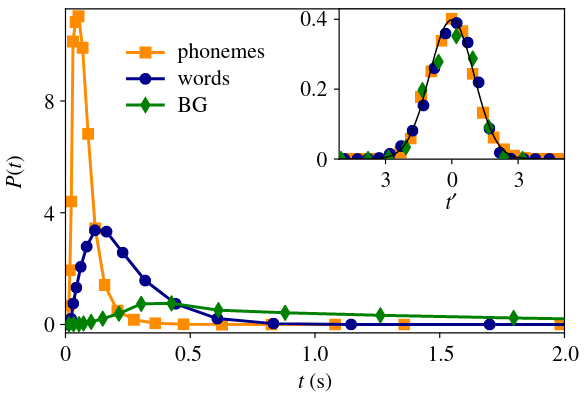
\includegraphics[width=0.7\textwidth,height=\textheight]{lognormal.png}
\caption{Distribuição lognormal na duração de fonemas, palavras e grupos
respiratórios no inglês (\protect\hyperlink{ref-Torre2019}{Torre et al.
2019}).\label{fig-lognormal}}
\end{figure}

\note{Dizemos uma v.a. \(X\) possui distribuição lognormal se o
logaritmo dela, \(Y=\ln(X)\), possuir distribuição normal. O gráfico
menor da figura \ref{fig-lognormal}, no canto superior direito,
apresenta o escalonamento dos valores para verificar que de fato seguem
uma distribuição normal.}
\end{frame}

\begin{frame}{Lei de Heaps/Herdan}
\protect\hypertarget{lei-de-heapsherdan}{}
A lei de Heaps/Herdan descreve o crescimento do vocabulário em um texto.

\[
V(n) = K n^\beta, \quad \beta < 1
\] \(K\) tipicamente está entre 10 e 100, e \(\beta\) entre \(0.4\) e
\(0.6\).
\end{frame}

\begin{frame}
\begin{figure}
\centering
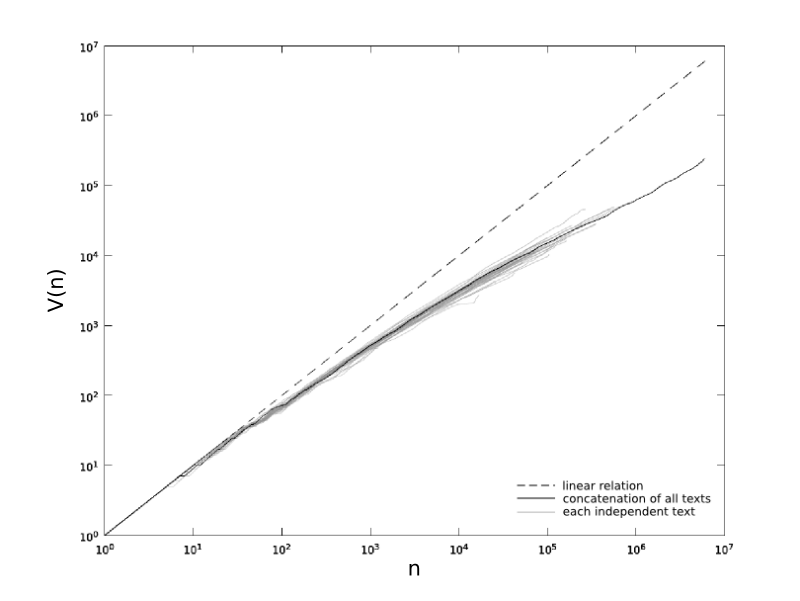
\includegraphics[width=0.7\textwidth,height=\textheight]{heaps.png}
\caption{Crescimento do vocabulário em 35 livros do projeto Gutenberg
(\protect\hyperlink{ref-leoca2013}{Araújo 2013}).}
\end{figure}
\end{frame}

\begin{frame}
Leijenhorst, Weide, e Grootjen
(\protect\hyperlink{ref-vanLeijenhorst2005}{2005}) mostra que é possível
derivar matematicamente a lei de Heaps a partir da lei de Zipf. Nesta
caso, teremos \(\beta = 1/\alpha\), sendo necessário \(\alpha > 1\).
\end{frame}

\begin{frame}
\begin{figure}
\centering
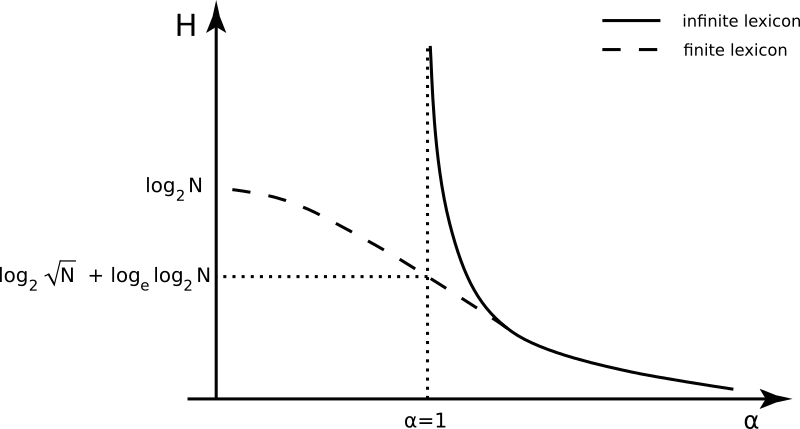
\includegraphics[width=0.7\textwidth,height=\textheight]{entropy_zipf.png}
\caption{Entropia para uma fonte com distribuição de Zipf. Comparação
entre léxico finito e infinito
(\protect\hyperlink{ref-mandelbrot1953theorie}{Benoit Mandelbrot 1953};
\protect\hyperlink{ref-leoca2013glotto}{Araújo, Silva, e Yehia 2013}).}
\end{figure}
\end{frame}

\begin{frame}{Crescimento do vocabulário e das classes de baixa
frequência}
\protect\hypertarget{crescimento-do-vocabuluxe1rio-e-das-classes-de-baixa-frequuxeancia}{}
A lei de potência proposta por Altmann \(y = Ax^{-b}\) descreve bem a
relação entre crescimento do vocabulário e tamanho das classes.

\begin{figure}
\centering
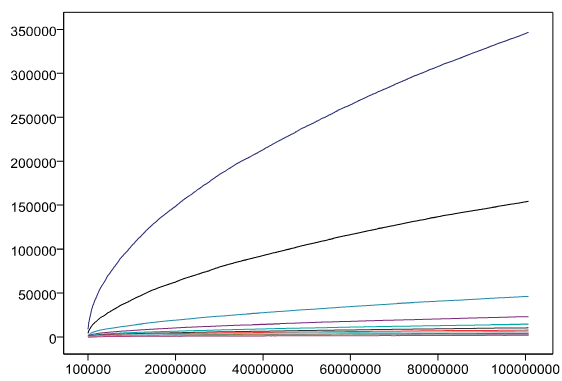
\includegraphics[width=0.5\textwidth,height=\textheight]{classsizegrowth.png}
\caption{Crescimento do vocabulário e das classes de baixa frequência (1
a 15) (\protect\hyperlink{ref-fan2014some}{Fan, Wang, e Gao 2014}).}
\end{figure}
\end{frame}

\begin{frame}{Lei de Zipf inversa}
\protect\hypertarget{lei-de-zipf-inversa}{}
Zipf (\protect\hyperlink{ref-zipf1935}{1935}) estabelece a lei inversa,
relacionando a frequência de ocorrência e o número de palavras para uma
dada frequência.

\[
N_f = a f^{-b}
\]

onde \(f\) é a frequência de ocorrência e \(N_f\) o número de palavras
com uma dada frequência de ocorrência \(f\).
\end{frame}

\begin{frame}
\begin{figure}
\centering
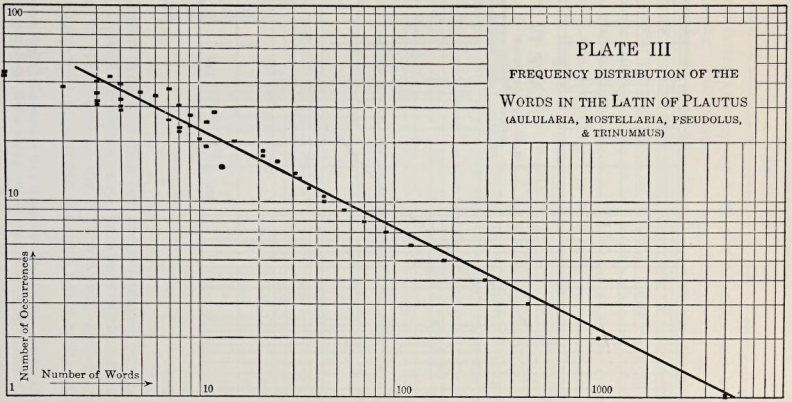
\includegraphics[width=0.8\textwidth,height=\textheight]{zipf-inverse.png}
\caption{Relação entre frequência de ocorrência e número de palavras
para uma dada frequência (\protect\hyperlink{ref-zipf1935}{Zipf 1935}).}
\end{figure}
\end{frame}

\begin{frame}
\begin{figure}
\centering
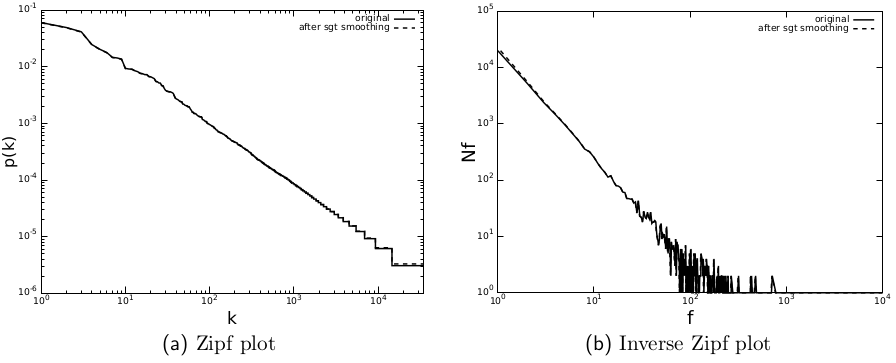
\includegraphics[width=0.8\textwidth,height=\textheight]{zipf-inverse-2.png}
\caption{Gráfico de Zipf e gráfico inverso para o texto Ulysses
(\protect\hyperlink{ref-leoca2013}{Araújo 2013}).}
\end{figure}
\end{frame}

\begin{frame}{Hapax Legomena}
\protect\hypertarget{hapax-legomena}{}
O número de hapax legomena algumas vezes é utilizado como uma medida de
riqueza de vocabulário.

O número de hapax legomena (HL) e o tamanho do vocabulário (V)
apresentam uma relação linear

\[
HL = aV - b
\]
\end{frame}

\begin{frame}
\begin{figure}
\centering
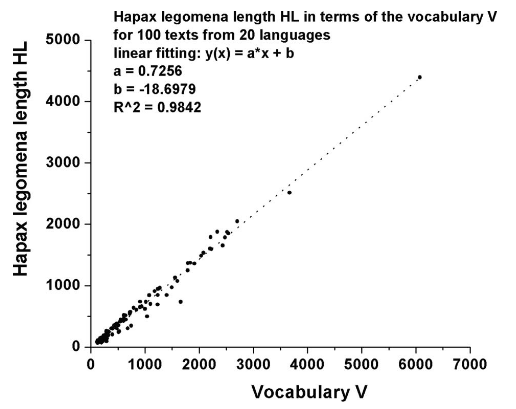
\includegraphics[width=0.6\textwidth,height=\textheight]{altmann-hapaxlegomena.png}
\caption{Dependência entre o número de hapax legomena (HL) e o tamanho
do vocabulário (V) (\protect\hyperlink{ref-popescu2008}{Popescu e
Altmann 2008}).}
\end{figure}
\end{frame}

\begin{frame}
\begin{figure}
\centering
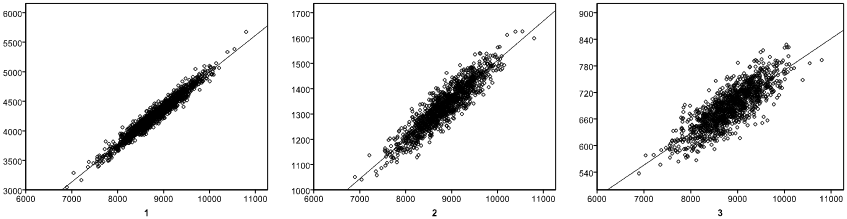
\includegraphics[width=1\textwidth,height=\textheight]{fan2014-richness.png}
\caption{Relação entre o tamanho do vocabulário e o tamanho das classes
de baixa frequência (1, 2 e 3). Para esta análise, o British National
Corpus foi dividido em 1.000 pedaços de aproximadamente 100.000
palavras. (\protect\hyperlink{ref-fan2014some}{Fan, Wang, e Gao 2014}).}
\end{figure}
\end{frame}

\begin{frame}
A razão entre o tamanho do vocabulário e o número de hapaxes foi objeto
de estudo de diversos linguistas
(\protect\hyperlink{ref-baayen1996effects}{H. Baayen 1996};
\protect\hyperlink{ref-tweedie1998variable}{Tweedie e Baayen 1998};
\protect\hyperlink{ref-baayen2001word}{R. H. Baayen 2001};
\protect\hyperlink{ref-kornai2002many}{Kornai 2002};
\protect\hyperlink{ref-fengxiang2010asymptotic}{Fengxiang 2010}).
\end{frame}

\begin{frame}{Lei de Menzerath-Altmann}
\protect\hypertarget{lei-de-menzerath-altmann}{}
Menzerath (\protect\hyperlink{ref-menzerath1954}{1954}) observou a
existência de uma relação inversa entre o tamanho de um construto e o
tamanho de seus constituintes.

\begin{figure}
\centering
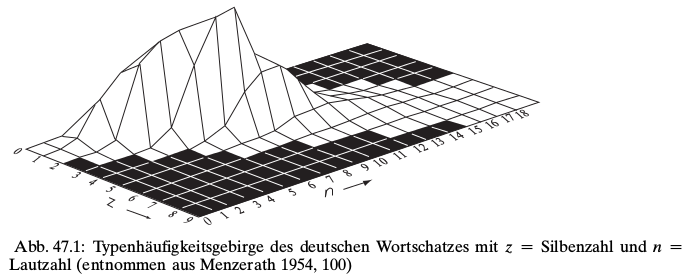
\includegraphics[width=0.7\textwidth,height=\textheight]{menzerath-fig471.png}
\caption{Frequencia de tipo das palavras alemãs em relação ao número de
sílabas (\(z\)) e o número de sons (\(n\))
(\protect\hyperlink{ref-menzerath1954}{Menzerath 1954}).}
\end{figure}
\end{frame}

\begin{frame}
\begin{figure}
\centering
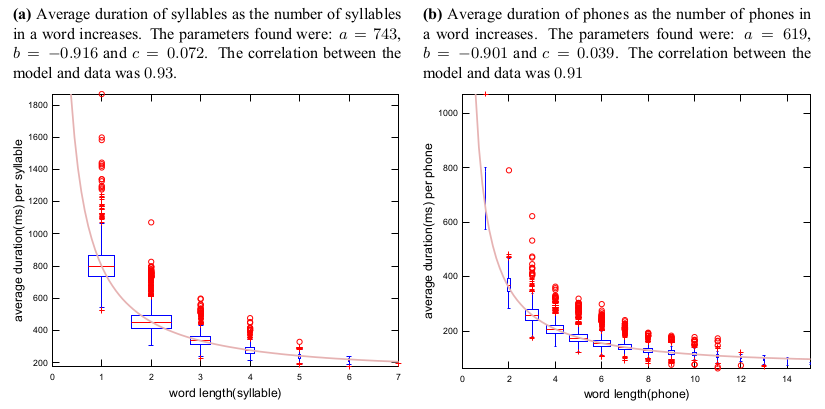
\includegraphics[width=0.8\textwidth,height=\textheight]{leolca-menzerath.png}
\caption{Relação entre o comprimento das palavras e a duração de seus
constituintes. Foram analisadas 10.086 palavras do inglês, com dados
obtidos de dicionários online
(\protect\hyperlink{ref-araujo2014menzerath}{L. Araujo,
Cristófaro-Silva, e Yehia 2014}).}
\end{figure}
\end{frame}

\begin{frame}
\begin{figure}
\centering
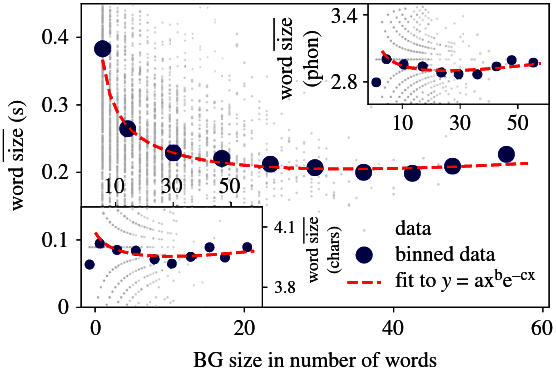
\includegraphics[width=0.7\textwidth,height=\textheight]{menzerath_bg.png}
\caption{Lei de Menzerath-Altmann. Relação entre o tamnho de grupo
respiratório (número de palavas) versus tamanho médio das palavras
(duração, número de fonemas, número de caracteres)
(\protect\hyperlink{ref-Torre2019}{Torre et al. 2019}).}
\end{figure}
\end{frame}

\begin{frame}
Altmann (\protect\hyperlink{ref-altmann1980}{1980}) observou que o
conceito de \textit{tamanho} poderia referir-se também à complexidade e
numero de elementos utilizados na composição. Altmann
(\protect\hyperlink{ref-altmann1980}{1980}) propôs o modelo matemático

\[
\frac{y'}{y} = \frac{b}{x} + c 
\]

para o qual a solução é

\[
y = a x^b e^{cx}
\]
\end{frame}

\begin{frame}
Para Köhler (\protect\hyperlink{ref-kohler1989menzerathsche}{1989}), a
lei de Menzerath-Altmann é uma manifestação característica de sistemas
complexos.

Outros estudos analizam a lei de Menzerath-Altmann em textos
(\protect\hyperlink{ref-hrebicek1995}{Hřebíček 1995};
\protect\hyperlink{ref-andres2010}{Andres 2010};
\protect\hyperlink{ref-araujo2020}{L. C. Araujo, Benevides, e Pereira
2020}; \protect\hyperlink{ref-gtorre2021}{Torre, Dębowski, e
Hernández-Fernández 2021}), fala {[}Hernández-Fernández, Torre, et al.
(\protect\hyperlink{ref-HernndezFernndez2019}{2019});Torre2019{]},
genoma (\protect\hyperlink{ref-ferrer2014menzerath}{Ramon
Ferrer-i-Cancho et al. 2014}), música
(\protect\hyperlink{ref-boroda1991}{Boroda e Altmann 1991}), comunicação
gestual de chipanzés (\protect\hyperlink{ref-heesen2019}{Heesen et al.
2019}), etc.
\end{frame}

\begin{frame}{Lei de Piotrowski-Altmann}
\protect\hypertarget{lei-de-piotrowski-altmann}{}
As línguas mudam pela interação entre formas antigas e novas.

Mudanças qualitativas: mudanças em entidades individuais, mudanças
sonoras. Mudanças em volume: crescimento/decaimento lexical.

O influxo de novos elementos em uma língua, ao longo do tempo, é
descrito por \[
p(t) = \frac{c}{1 + ae^{-bt}}
\]

(\protect\hyperlink{ref-altmann1983piotrowski}{Altmann 1983b},
\protect\hyperlink{ref-altmann1983law}{1983a};
\protect\hyperlink{ref-best2016bibliography}{Karl-Heinz Best 2016a};
\protect\hyperlink{ref-stachowski2020}{Stachowski 2020})

Karl-Heinz Best (\protect\hyperlink{ref-Best2016}{2016b}) reúne uma
extensa lista de publicações sobre a lei de Piotrowski.
\end{frame}

\begin{frame}
\begin{figure}
\centering
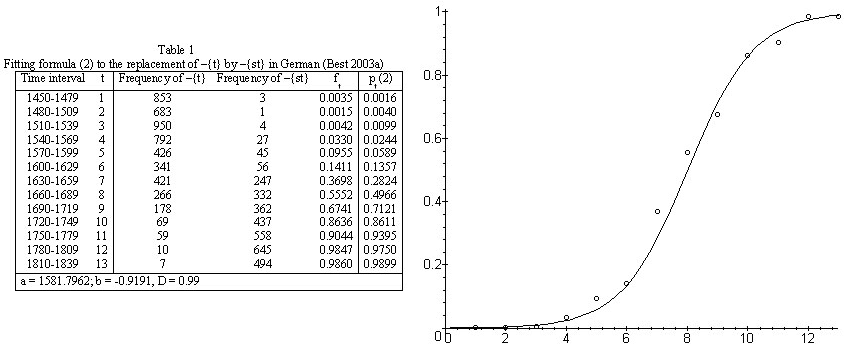
\includegraphics[width=1\textwidth,height=\textheight]{best_german_wollen.png}
\caption{Substituição de -\{t\} por -\{st\} na 2a pessoa do singular do
presente do indicativo no verbo alemão `wollen' (\emph{wilt} →
\emph{willst}) (\protect\hyperlink{ref-best2006quantitative}{K. H. Best
2006}).}
\end{figure}
\end{frame}

\begin{frame}
\begin{figure}
\centering
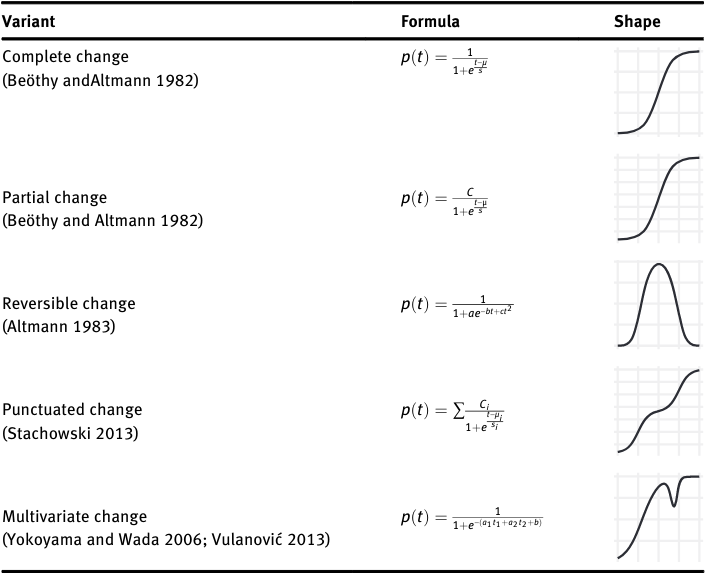
\includegraphics[width=0.7\textwidth,height=\textheight]{stachowski2020-fig1.png}
\caption{Variantes da lei Piotrowski-Altmann
(\protect\hyperlink{ref-stachowski2020}{Stachowski 2020}).}
\end{figure}

\note{A variante da \textbf{mudança completa} é a mais básica,
descrevendo a substituição completa de uma forma por outra. Exemplo:
desaparecimento do sufixo -ov do plural genitivo dos nomes de unidades
nos textos técnicos russos entre 1880 e 1920. A \textbf{mudança parcial}
descreve mudanças que devem ser descritas pelo volume ao invés de
percentual. Por exemplo: empréstimos de outras línguas no alemão. A
variante de \textbf{mudança reversível} descreve uma mudança que se
inicia, tem um pico e reverte-se. Por exemplo: epêntese do -e em verbos
fortes no alemão.}

\note{Starke Verben haben in der 1. Person Singular Präteritum Indikativ
keine Endung -e: ich ging (gehen), sah (sehen), kam (kommen), nahm
(nehmen), fand (finden), half (helfen), blieb (bleiben), \ldots{} Die
Ausnahme ist werden: ich wurde (veraltet: ward)

Die e-Epithese bei den starken Verben ist ein Sprachwandelprozeß, der
sich nicht durchgesetzt hat. Im Verlauf des 17. Jahrhunderts erlangte
sie ihre größte Beliebtheit, war jedoch nie obligatorisch. Man findet
also auch in ihrer Hochzeit bei ein und demselben Autor Formen ohne -e
neben solchen mit -e. Die Formen mit -e sind immer seltener als die
ohne.

\url{https://german.stackexchange.com/questions/48263/die-form-fande-als-1-person-singular-pr\%c3\%a4teritum-indikativ-e-epithese}}
\end{frame}

\begin{frame}{Lei de Frumkina}
\protect\hypertarget{lei-de-frumkina}{}
A lei de Frumkina (lei dos blocos de texto) descreve a frequência de
ocorrência de certas unidades linguísticas em blocos de texto. A
distribuição hipergeométrica negativa é um bom modelo para descrever a
ocorrência (\protect\hyperlink{ref-altmann1982towards}{Altmann e
Burdinski 1982}; \protect\hyperlink{ref-best2005sprachliche}{Karl-Heinz
Best 2005}; \protect\hyperlink{ref-textblockgesetz2021}{Wikipedia
2021b}).
\end{frame}

\begin{frame}
\begin{figure}
\centering
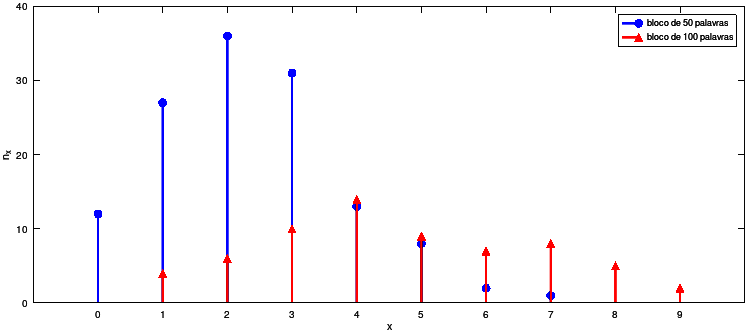
\includegraphics[width=0.7\textwidth,height=\textheight]{frumkina-a.png}
\caption{Ocorrências de ``a'' no capítulo 1 de \emph{Die Bäder von
Lucca} (Heinrich Heine) com blocos de tamanho 50 e 100
(\protect\hyperlink{ref-best2005sprachliche}{Karl-Heinz Best 2005}).}
\end{figure}
\end{frame}

\begin{frame}{Lei de Martin}
\protect\hypertarget{lei-de-martin}{}
A lei de Martin diz respeito à estruturação hierárquica do léxico.

~

Exemplo:

Sessel(1) -- Sitzmöbel(2) -- Möbel(3) -- Einrichtungsgegenstand(4) --
Gegenstand(5)

(Poltrona - móveis de assento - móveis - item de decoração - objeto)

\note{A posição que uma palavra ocupa na cadeia lexical diz respeito a
quantas definições são ligadas a ela, indo do termo mais específico ao
mais geral, formando uma hierarquia de significados cada vez mais
gerais. O número de definições diminui com o aumento da generalidade.}
\end{frame}

\begin{frame}
\begin{figure}
\centering
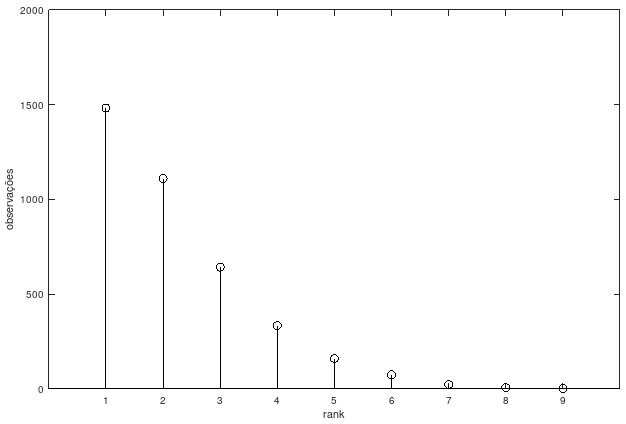
\includegraphics[width=0.7\textwidth,height=\textheight]{martins.png}
\caption{A distribuição de Poisson mista é um bom modelo para os dados
de Bagheri (\protect\hyperlink{ref-bagheri2002}{2002};
\protect\hyperlink{ref-martinschesgesetz2021}{Wikipedia 2021a})}
\end{figure}
\end{frame}

\hypertarget{softwares}{%
\section{Softwares}\label{softwares}}

\begin{frame}{Altmann-Fitter}
\protect\hypertarget{altmann-fitter}{}
\begin{figure}
\centering
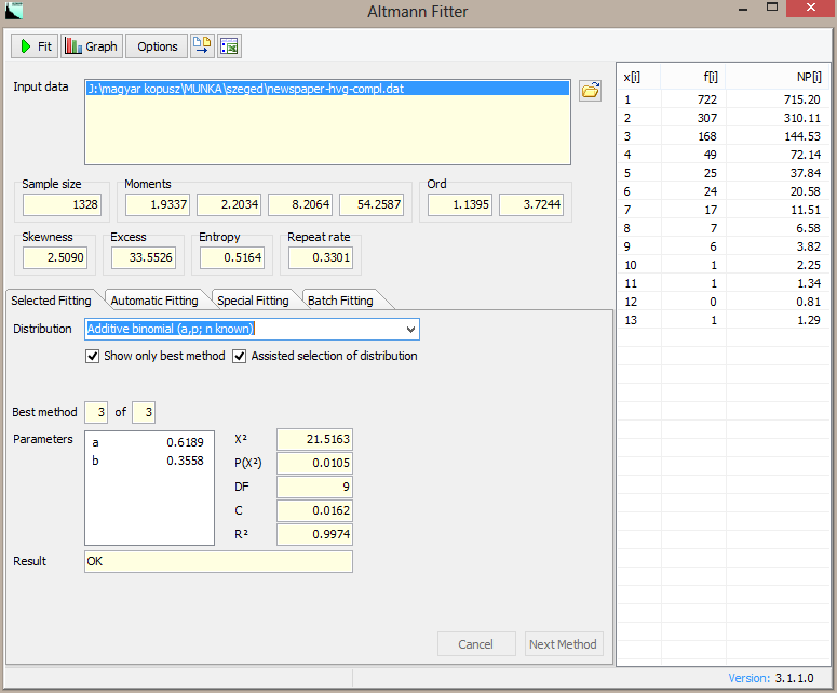
\includegraphics[width=0.5\textwidth,height=\textheight]{altmannfitter.png}
\caption{Tela do software Altmann-Fitter.}
\end{figure}

\note{O Altmann Fitter é um software interativo para ajuste de
distribuições de probabilidade discretas a dados de frequência. O
algoritmo utilizado é baseado no Nelder-Mead Simplex. Mais de 200
distribuições estão definidas e implementadas no software. Os
procedimentos matemáticos são automatizados. O software iterativamente
busca melhor o ajuste, buscando a distribuição que melhor se explique os
dados observados.}
\end{frame}

\begin{frame}
\begin{figure}
\centering
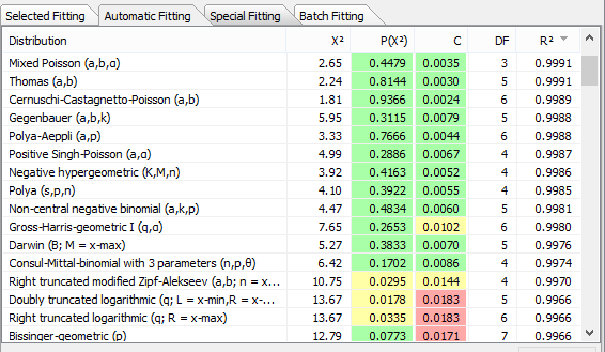
\includegraphics[width=0.7\textwidth,height=\textheight]{altmannfitter2.png}
\caption{Tela do software Altmann-Fitter.}
\end{figure}
\end{frame}

\begin{frame}
\begin{figure}
\centering
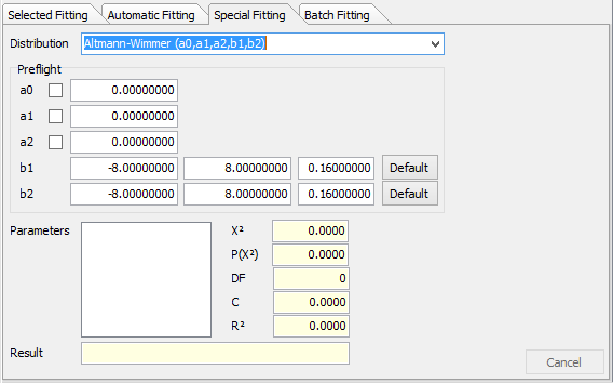
\includegraphics[width=0.7\textwidth,height=\textheight]{altmannfitter3.png}
\caption{Tela do software Altmann-Fitter.}
\end{figure}
\end{frame}

\begin{frame}{R}
\protect\hypertarget{r}{}
Pacotes

\begin{description}
\tightlist
\item[languageR]
Analyzing Linguistic Data: A Practical Introduction to Statistics

Autores: R. H. Baayen, Elnaz Shafaei-Bajestan

\url{https://cran.r-project.org/web/packages/languageR/}
\item[zipfR]
Statistical Models for Word Frequency Distributions

Autores: Stefan Evert, Marco Baroni

\url{https://cran.r-project.org/web/packages/zipfR/}
\item[fitdistrplus]
Help to Fit of a Parametric Distribution to Non-Censored or Censored
Data

Autores: Marie-Laure Delignette-Muller, Christophe Dutang, Regis
Pouillot, Jean-Baptiste Denis, Aurelie Siberchicot

\url{https://cran.r-project.org/web/packages/fitdistrplus/}
\end{description}
\end{frame}

\hypertarget{teoria-1}{%
\section{Teoria}\label{teoria-1}}

\begin{frame}{Construção de uma teoria}
\protect\hypertarget{construuxe7uxe3o-de-uma-teoria}{}
Abordagens:

\begin{enumerate}
\tightlist
\item
  linguística sinergética
\item
  teoria unificada
\end{enumerate}

\note{As leis da linguística quantitativa são observadas na comunicação
escrita, na comunicação oral, em certos aspectos da comunicação animal
e, algumas vezes, também em outros fenômenos da natureza. Certas podem
ser ligadas à emergência em sistemas complexos, aspectos associados à
sistemas de comunicação, ou aspectos cognitivos e psicológicos que devem
ser explorados.

\begin{enumerate}
\tightlist
\item
  A proposta sinergética busca integrar as leis e hipóteses em um modelo
  complexo para descrever o fenômeno linguístico. Utilizam para tanto um
  axioma central: as línguas são sistemas auto-organizativos. Estabelece
  também alguns requisitos que devem ser seguidos por um sistema
  semiótico: ser possível realizar codificação e decodificação com
  eficiência, economia de memória, minimização de esforço, dentre
  outros.
\item
  A teoria unificada busca integrar as leis e hipóteses a partir de
  equações diferenciais gerais (ou equações de diferenças, no caso
  discreto), assim como dois pressupostos gerais: 1) a dinâmica de uma
  variável linguística \(y\) será modelada matematicamente em termos de
  sua mudança relativa \((dy/y)\); 2) uma outra variável \(x\) que tenha
  efeito sobre \(y\) deverá ser considerada da mesma forma em temos de
  sua mudança relativa \((dx/x)\).
\end{enumerate}}
\end{frame}

\hypertarget{references}{%
\section*{References}\label{references}}
\addcontentsline{toc}{section}{References}

\begin{frame}[allowframebreaks]{References}
\hypertarget{refs}{}
\begin{CSLReferences}{1}{0}
\leavevmode\vadjust pre{\hypertarget{ref-suzuki2005}{}}%
Abe, Sumiyoshi, e Norikazu Suzuki. 2005. {"Scale-free statistics of time
interval between successive earthquakes"}. \emph{Physica A: Statistical
Mechanics and its Applications} 350 (2): 588--96.

\leavevmode\vadjust pre{\hypertarget{ref-huberman2002}{}}%
Adamic, Lada A., e Bernardo A. Huberman. 2002. {"Zipf's law and the
Internet"}. \emph{Glottometrics} 3: 143--50.

\leavevmode\vadjust pre{\hypertarget{ref-altmann1980}{}}%
Altmann, Gabriel. 1980. {"Prolegomena to {M}enzerath's law"}.
\emph{Glottometrika} 2: 1--10.

\leavevmode\vadjust pre{\hypertarget{ref-altmann1983law}{}}%
---------. 1983a. {"A Law of Change in Language, Historical
Linguistics"}. \emph{Quantitative Linguistics} 18: 104--15.

\leavevmode\vadjust pre{\hypertarget{ref-altmann1983piotrowski}{}}%
---------. 1983b. {"Das Piotrowski-Gesetz und seine
Verallgemeinerungen"}. \emph{Exakte Sprachwandelforschung}, 54--90.

\leavevmode\vadjust pre{\hypertarget{ref-altmann1982towards}{}}%
Altmann, Gabriel, e Violetta Burdinski. 1982. {"Towards a law of word
repetitions in text-blocks"}. \emph{Glottometrika} 4: 147--67.

\leavevmode\vadjust pre{\hypertarget{ref-andres2010}{}}%
Andres, Jan. 2010. {"On a Conjecture about the Fractal Structure of
Language"}. \emph{Journal of Quantitative Linguistics} 17 (2): 101--22.
\url{https://doi.org/10.1080/09296171003643189}.

\leavevmode\vadjust pre{\hypertarget{ref-araujo2020}{}}%
Araujo, Leonardo Carneiro, Aline Benevides, e Marcos Pereira. 2020.
{"An{á}lise da Lei de Menzerath no Portugu{ê}s Brasileiro"}.
\emph{Linguam{á}tica} 12 (1): 31--48.
\url{https://doi.org/10.21814/lm.12.1.300}.

\leavevmode\vadjust pre{\hypertarget{ref-araujo2014menzerath}{}}%
Araujo, Leonardo, Thaı̈s Cristófaro-Silva, e Hani Yehia. 2014.
{"Menzerath's law on word duration"}. Em \emph{1st International DINAFON
Meeting}.

\leavevmode\vadjust pre{\hypertarget{ref-leoca2013}{}}%
Araújo, Leonardo Carneiro de. 2013. {"Statistical analyses in language
usage"}. Tese de doutorado, Universidade Federal de Minas Gerais.

\leavevmode\vadjust pre{\hypertarget{ref-leoca2013glotto}{}}%
Araújo, Leonardo Carneiro de, Thaı̈s Cristófaro Silva, e Hani C. Yehia.
2013. {"Entropy of a Zipfian Distributed Lexicon"}. \emph{Glottometrics}
26: 38--49.

\leavevmode\vadjust pre{\hypertarget{ref-baayen1996effects}{}}%
Baayen, Harald. 1996. {"The effects of lexical specialization on the
growth curve of the vocabulary"}. \emph{Computational Linguistics} 22
(4): 455--80.

\leavevmode\vadjust pre{\hypertarget{ref-baayen2001word}{}}%
Baayen, R Harald. 2001. \emph{Word frequency distributions}. Vol. 18.
Springer Science \& Business Media.

\leavevmode\vadjust pre{\hypertarget{ref-baek2011zipf}{}}%
Baek, Seung Ki, Sebastian Bernhardsson, e Petter Minnhagen. 2011.
{"Zipf's law unzipped"}. \emph{New Journal of Physics} 13 (4): 043004.

\leavevmode\vadjust pre{\hypertarget{ref-bagheri2002}{}}%
Bagheri, Dariusch. 2002. {"Definitionsfolgen und Lexemnetze"}. Em
\emph{Einführung in die quantitative Lexikologie}, editado por Gabriel
Altmann, Dariusch Bagheri, Hans Goebl, Reinhard Köhler, e Claudia Prün,
124. Peust \& Gutschmidt.

\leavevmode\vadjust pre{\hypertarget{ref-Baixeries2013}{}}%
Baixeries, Jaume, Brita Elvevåg, e Ramon Ferrer-i-Cancho. 2013. {"The
Evolution of the Exponent of Zipf{\textquotesingle}s Law in Language
Ontogeny"}. Editado por Satoru Hayasaka. \emph{{PLoS} {ONE}} 8 (3):
e53227. \url{https://doi.org/10.1371/journal.pone.0053227}.

\leavevmode\vadjust pre{\hypertarget{ref-perbak}{}}%
Bak, Per. 1996. \emph{How Nature Works: the science of self-organized
criticality}. Copernicus.

\leavevmode\vadjust pre{\hypertarget{ref-bentz2016zipf}{}}%
Bentz, Chris, e Ramon Ferrer Cancho. 2016. {"Zipf's law of abbreviation
as a language universal"}. Em \emph{Proceedings of the Leiden workshop
on capturing phylogenetic algorithms for linguistics}, 1--4. University
of T{ü}bingen.

\leavevmode\vadjust pre{\hypertarget{ref-best2006quantitative}{}}%
Best, K. H. 2006. \emph{Quantitative Linguistik: eine Ann{ä}herung}.
G{ö}ttinger linguistische Abhandlungen. Peust \& Gutschmidt.
\url{https://books.google.com.br/books?id=/_iCwMQAACAAJ}.

\leavevmode\vadjust pre{\hypertarget{ref-best2005sprachliche}{}}%
Best, Karl-Heinz. 2005. {"Sprachliche Einheiten in Textbl{ö}cken."}
\emph{Glottometrics} 9: 1--12.

\leavevmode\vadjust pre{\hypertarget{ref-best2016bibliography}{}}%
---------. 2016a. {"Bibliography--Piotrowski's law"}.
\emph{Glottotheory} 7 (1): 89--93.

\leavevmode\vadjust pre{\hypertarget{ref-Best2016}{}}%
---------. 2016b. {"Bibliography {\textendash} Piotrowski's law"}.
\emph{Glottotheory} 7 (1). \url{https://doi.org/10.1515/glot-2016-0006}.

\leavevmode\vadjust pre{\hypertarget{ref-Bian2016}{}}%
Bian, Chunhua, Ruokuang Lin, Xiaoyu Zhang, Qianli D. Y. Ma, e Plamen Ch.
Ivanov. 2016. {"Scaling laws and model of words organization in spoken
and written language"}. \emph{{EPL} (Europhysics Letters)} 113 (1):
18002. \url{https://doi.org/10.1209/0295-5075/113/18002}.

\leavevmode\vadjust pre{\hypertarget{ref-boroda1991}{}}%
Boroda, M., e Gabriel Altmann. 1991. {"Menzerath's law in musical
texts"}. \emph{Musikometrica} 3: 1--13.

\leavevmode\vadjust pre{\hypertarget{ref-cancho2005decoding}{}}%
Cancho, Ramon Ferrer i. 2005. {"Decoding least effort and scaling in
signal frequency distributions"}. \emph{Physica A: Statistical Mechanics
and its Applications} 345 (1-2): 275--84.

\leavevmode\vadjust pre{\hypertarget{ref-cancho2007}{}}%
---------. 2007. {"On the universality of Zipf's law for word
frequencies"}. Em \emph{Exact Methods in the Study of Language and
Text}, editado por Peter Grzybek e Reinhard Köhler, 131--40. De Gruyter
Mouton. \url{https://doi.org/10.1515/9783110894219.131}.

\leavevmode\vadjust pre{\hypertarget{ref-cancho2003}{}}%
Cancho, Ramon Ferrer i, e Ricard V. Solé. 2003. {"Least effort and the
origins of scaling in human language"}. \emph{Proceedings of the
National Academy of Sciences} 100 (3): 788--91.
\url{https://doi.org/10.1073/pnas.0335980100}.

\leavevmode\vadjust pre{\hypertarget{ref-chater1999scale}{}}%
Chater, Nick, e Gordon DA Brown. 1999. {"Scale-invariance as a unifying
psychological principle"}. \emph{Cognition} 69 (3): B17--24.

\leavevmode\vadjust pre{\hypertarget{ref-choi2005}{}}%
Choi, JS, Kyungsik Kim, SM Yoon, KH Chang, e C Christopher Lee. 2005.
{"Zipf's law distributions in Korean financial markets"}. \emph{Journal
of the Korean Physical Society} 47 (1): 171.

\leavevmode\vadjust pre{\hypertarget{ref-conrad2004power}{}}%
Conrad, Brian, e Michael Mitzenmacher. 2004. {"Power laws for monkeys
typing randomly: the case of unequal probabilities"}. \emph{IEEE
Transactions on information theory} 50 (7): 1403--14.

\leavevmode\vadjust pre{\hypertarget{ref-corominas2010universality}{}}%
Corominas-Murtra, Bernat, e Ricard V Solé. 2010. {"Universality of
Zipf's law"}. \emph{Physical Review E} 82 (1): 011102.

\leavevmode\vadjust pre{\hypertarget{ref-cox}{}}%
Cox, Raymond A K, James M. Felton, e Kee C. Chung. 1995. {"The
concentration of commercial success in popular music: an analysis of the
distribution of gold records"}. \emph{Journal of Cultural Economics} 19:
333--40.

\leavevmode\vadjust pre{\hypertarget{ref-crovella96}{}}%
Crovella, Marl E., e Azer Bestavros. 1996. {"Self-Similarity in {W}orld
{W}ide {W}eb Traffic: Evidence and Possible Causes"}. Em
\emph{Proceedings of the 1996 ACM SIGMETRICS International Conference on
Measurement and Modeling of Computer Systems}, 160--69.
\url{http://www.cs.bu.edu/faculty/crovella/paper-archive/self-sim/sigmetrics-version.ps}.

\leavevmode\vadjust pre{\hypertarget{ref-fan2014some}{}}%
Fan, Fengxiang, Yaqin Wang, e Zhao Gao. 2014. {"Some macro quantitative
features of low-frequency word classes."} \emph{Glottometrics} 28:
1--12.

\leavevmode\vadjust pre{\hypertarget{ref-farmer2008power}{}}%
Farmer, J Doyne, e John Geanakoplos. 2008. {"Power laws in economics and
elsewhere"}. Em \emph{Santa Fe Institute}.

\leavevmode\vadjust pre{\hypertarget{ref-fengxiang2010asymptotic}{}}%
Fengxiang, Fan. 2010. {"An asymptotic model for the English
hapax/vocabulary ratio"}. \emph{Computational Linguistics} 36 (4):
631--37.

\leavevmode\vadjust pre{\hypertarget{ref-cancho2005hidden}{}}%
Ferrer-i-Cancho, R. 2005. {"Hidden communication aspects inside the
exponent of Zipf's law"}. \emph{Glottometrics} 11 (janeiro): 96--117.

\leavevmode\vadjust pre{\hypertarget{ref-ferrer2014menzerath}{}}%
Ferrer-i-Cancho, Ramon, Antoni Hernández-Fernández, Jaume Baixeries,
Łukasz Dębowski, e Ján Mačutek. 2014. {"When is Menzerath-Altmann law
mathematically trivial? A new approach"}. \emph{Statistical applications
in genetics and molecular biology} 13 (6): 633--44.

\leavevmode\vadjust pre{\hypertarget{ref-cancho2013compression}{}}%
Ferrer-i-Cancho, Ramon, Antoni Hernández-Fernández, David Lusseau,
Govindasamy Agoramoorthy, Minna J Hsu, e Stuart Semple. 2013.
{"Compression as a universal principle of animal behavior"}.
\emph{Cognitive Science} 37 (8): 1565--78.

\leavevmode\vadjust pre{\hypertarget{ref-cancho2018origins}{}}%
Ferrer-i-Cancho, Ramon, e Michael S Vitevitch. 2018. {"The origins of
Zipf's meaning-frequency law"}. \emph{Journal of the Association for
Information Science and Technology} 69 (11): 1369--79.

\leavevmode\vadjust pre{\hypertarget{ref-fujiwara2004}{}}%
Fujiwara, Yoshi. 2004. {"Zipf law in firms bankruptcy"}. \emph{Physica
A: Statistical and Theoretical Physics} 337 (1-2): 219--30.

\leavevmode\vadjust pre{\hypertarget{ref-furusawa}{}}%
Furusawa, Chikara, e Kunihiko Kaneko. 2003. {"Zipf's law in gene
expression"}. \emph{Physical review letters} 90 (8): 088102.

\leavevmode\vadjust pre{\hypertarget{ref-gabaix1999}{}}%
Gabaix, Xavier. 1999. {"Zipf's Law for Cities: An Explanation"}.
\emph{Quarterly Journal of Economics} 114 (3): 739--67.

\leavevmode\vadjust pre{\hypertarget{ref-gopinath2008modeling}{}}%
Gopinath, Deepa P, S Veena, e Achuthsankar S Nair. 2008. {"Modeling of
vowel duration in Malayalam speech using probability distribution"}.
\emph{Proceedings of the speech prosody, Campinas, Brazil}, 6--9.

\leavevmode\vadjust pre{\hypertarget{ref-grimes2000}{}}%
Grimes, Barbara F. 2000. {"Ethnologue: Languages of the World"}. Texas:
\url{https://www.ethnologue.com/14/}; SIL International.

\leavevmode\vadjust pre{\hypertarget{ref-guiraud1968semic}{}}%
Guiraud, Pierre. 1968. {"The semic matrices of meaning"}. \emph{Social
science information} 7 (2): 131--39.

\leavevmode\vadjust pre{\hypertarget{ref-heesen2019}{}}%
Heesen, Raphaela, Catherine Hobaiter, Ramon Ferrer-i-Cancho, e Stuart
Semple. 2019. {"Linguistic laws in chimpanzee gestural communication"}.
\emph{Proceedings of the Royal Society B: Biological Sciences} 286
(1896): 20182900. \url{https://doi.org/10.1098/rspb.2018.2900}.

\leavevmode\vadjust pre{\hypertarget{ref-herdan1958relation}{}}%
Herdan, Gustav. 1958. {"The relation between the dictionary distribution
and the occurrence distribution of word length and its importance for
the study of quantitative linguistics"}. \emph{Biometrika} 45 (1-2):
222--28.

\leavevmode\vadjust pre{\hypertarget{ref-hernandez2016testing}{}}%
Hernández-Fernández, Antoni, Bernardino Casas, Ramon Ferrer-i-Cancho, e
Jaume Baixeries. 2016. {"Testing the robustness of laws of polysemy and
brevity versus frequency"}. Em \emph{International Conference on
Statistical Language and Speech Processing}, 19--29. Springer.

\leavevmode\vadjust pre{\hypertarget{ref-hernandez2019linguistic}{}}%
Hernández-Fernández, Antoni, Iván G. Torre, Juan-Marı́a Garrido, e Lucas
Lacasa. 2019. {"Linguistic laws in speech: the case of Catalan and
Spanish"}. \emph{Entropy} 21 (12): 1153.

\leavevmode\vadjust pre{\hypertarget{ref-HernndezFernndez2019}{}}%
Hernández-Fernández, Antoni, Iván G. Torre, Juan-Marı́a Garrido, e Lucas
Lacasa. 2019. {"Linguistic Laws in Speech: The Case of Catalan and
Spanish"}. \emph{Entropy} 21 (12): 1153.
\url{https://doi.org/10.3390/e21121153}.

\leavevmode\vadjust pre{\hypertarget{ref-hernando2009zipf}{}}%
Hernando, A, D Puigdomènech, D Villuendas, C Vesperinas, e A Plastino.
2009. {"Zipf's law from a Fisher variational-principle"}. \emph{Physics
Letters A} 374 (1): 18--21.

\leavevmode\vadjust pre{\hypertarget{ref-hrebicek1995}{}}%
Hřebíček, Ludek. 1995. \emph{Text Levels. Language Constructs,
Constituents and the Menzerath-Altmann Law}. Quantitative linguistics.
Wissenschaftlicher Verlag Trier.

\leavevmode\vadjust pre{\hypertarget{ref-huffman1952method}{}}%
Huffman, David A. 1952. {"A method for the construction of
minimum-redundancy codes"}. \emph{Proceedings of the IRE} 40 (9):
1098--1101.

\leavevmode\vadjust pre{\hypertarget{ref-ilgen2007investigation}{}}%
Ilgen, Bahar, e Bahar Karaoglan. 2007. {"Investigation of Zipf's
`law-of-meaning'on Turkish corpora"}. Em \emph{2007 22nd international
symposium on computer and information sciences}, 1--6. IEEE.

\leavevmode\vadjust pre{\hypertarget{ref-ito1990earthquakes}{}}%
Ito, Keisuke, e Mitsuhiro Matsuzaki. 1990. {"Earthquakes as
self-organized critical phenomena"}. \emph{Journal of Geophysical
Research: Solid Earth} 95 (B5): 6853--60.

\leavevmode\vadjust pre{\hypertarget{ref-kanwal2017}{}}%
Kanwal, Jasmeen, Kenny Smith, Jennifer Culbertson, e Simon Kirby. 2017.
{"Zipf's Law of Abbreviation and the Principle of Least Effort: Language
users optimise a miniature lexicon for efficient communication"}.
\emph{Cognition} 165 (agosto): 45--52.
\url{https://doi.org/10.1016/j.cognition.2017.05.001}.

\leavevmode\vadjust pre{\hypertarget{ref-kawamura2002universality}{}}%
Kawamura, Kenji, e Naomichi Hatano. 2002. {"Universality of Zipf's
law"}. \emph{Journal of the Physical Society of Japan} 71 (5): 1211--13.

\leavevmode\vadjust pre{\hypertarget{ref-kohler1989menzerathsche}{}}%
Köhler, Reinhard. 1989. {"Das Menzerathsche Gesetz als Resultat des
Sprachverarbeitungsmechanismus"}. \emph{Das Menzerathsche Gesetz in
informations--verarbeitenden Systemen. Olms, Hildesheim}, 108--16.

\leavevmode\vadjust pre{\hypertarget{ref-kohli}{}}%
Kohli, Rajeev, e Raaj Kumar Sah. 2003. {"Market Shares: Some Power Law
Results and Observations"}. \emph{Management Science} 52 (11): 1792--98.

\leavevmode\vadjust pre{\hypertarget{ref-kornai2002many}{}}%
Kornai, András. 2002. {"How many words are there?"} \emph{Glottometrics}
4: 61--86.

\leavevmode\vadjust pre{\hypertarget{ref-vanLeijenhorst2005}{}}%
Leijenhorst, D. C. van, Th. P. van der Weide, e F. A. Grootjen. 2005.
{"A formal derivation of {H}eaps' Law"}. \emph{Information Sciences} 170
(2-4): 263--72.

\leavevmode\vadjust pre{\hypertarget{ref-li1992random}{}}%
Li, Wentian. 1992. {"Random texts exhibit Zipf's-law-like word frequency
distribution"}. \emph{IEEE Transactions on information theory} 38 (6):
1842--45.

\leavevmode\vadjust pre{\hypertarget{ref-mandelbrot1953theorie}{}}%
Mandelbrot, Benoit. 1953. \emph{Contribution {à} la th{é}orie
math{é}matique des jeux de communication}. Publications de l'Institut de
Statistique de l'Universit{é} de Par{ı́}s. Institut Henri Poincar{é}.

\leavevmode\vadjust pre{\hypertarget{ref-mandelbrot1966information}{}}%
---------. 1966. {"Information Theory and Psycholinguistics: A Theory of
Word Frequencies, Readings in Mathematical Social Sciences"}. MIT Press,
MA, USA.

\leavevmode\vadjust pre{\hypertarget{ref-mandelbrot1963}{}}%
Mandelbrot, Benoît. 1963. {"The Variation of Certain Speculative
Prices"}. \emph{The Journal of Business} 36 (4): 394--419.

\leavevmode\vadjust pre{\hypertarget{ref-mandelbrot1953}{}}%
Mandelbrot, Benoît B. 1953. {"An informational theory of the statistical
structure of languages"}. Em \emph{Communication Theory}, editado por
Betterworth W. Jackson, 486--502.

\leavevmode\vadjust pre{\hypertarget{ref-manin2008zipf}{}}%
Manin, Dmitrii Y. 2008. {"Zipf's law and avoidance of excessive
synonymy"}. \emph{Cognitive Science} 32 (7): 1075--98.

\leavevmode\vadjust pre{\hypertarget{ref-mccomas2014}{}}%
McComas, William F. 2014. {"Law (Scientific Law or Principle)"}. Em
\emph{The Language of Science Education: An Expanded Glossary of Key
Terms and Concepts in Science Teaching and Learning}, editado por
William F. McComas, 58--58. Rotterdam: SensePublishers.
\url{https://doi.org/10.1007/978-94-6209-497-0_51}.

\leavevmode\vadjust pre{\hypertarget{ref-mehri2017}{}}%
Mehri, Ali, e Maryam Jamaati. 2017. {"Variation of
Zipf{\textquotesingle}s exponent in one hundred live languages: A study
of the Holy Bible translations"}. \emph{Physics Letters A} 381 (31):
2470--77. \url{https://doi.org/10.1016/j.physleta.2017.05.061}.

\leavevmode\vadjust pre{\hypertarget{ref-menzerath1954}{}}%
Menzerath, Paul. 1954. \emph{Die Architektonik des deutschen
Wortschatzes}. Phonetische Studien. F. D{ü}mmler.

\leavevmode\vadjust pre{\hypertarget{ref-miller1957some}{}}%
Miller, George A. 1957. {"Some effects of intermittent silence"}.
\emph{The American journal of psychology} 70 (2): 311--14.

\leavevmode\vadjust pre{\hypertarget{ref-mitzenmacher2004brief}{}}%
Mitzenmacher, Michael. 2004. {"A brief history of generative models for
power law and lognormal distributions"}. \emph{Internet mathematics} 1
(2): 226--51.

\leavevmode\vadjust pre{\hypertarget{ref-moura2006zipf}{}}%
Moura Jr, Newton J, e Marcelo B Ribeiro. 2006. {"Zipf law for Brazilian
cities"}. \emph{Physica A: Statistical Mechanics and its Applications}
367: 441--48.

\leavevmode\vadjust pre{\hypertarget{ref-nicolis1989}{}}%
Nicolis, Grégoire, Cathy Nicolis, e John S. Nicolis. 1989. {"Chaotic
dynamics, {Markov} partitions, and {Zipf}'s law"}. \emph{Journal of
Statistical Physics} 54 (3--4): 915--24.

\leavevmode\vadjust pre{\hypertarget{ref-parker1956theory}{}}%
Parker-Rhodes, AF, e T Joyce. 1956. {"A theory of word-frequency
distribution"}. \emph{Nature} 178 (4545): 1308--8.

\leavevmode\vadjust pre{\hypertarget{ref-piantadosi2011word}{}}%
Piantadosi, Steven T, Harry Tily, e Edward Gibson. 2011. {"Word lengths
are optimized for efficient communication"}. \emph{Proceedings of the
National Academy of Sciences} 108 (9): 3526--29.

\leavevmode\vadjust pre{\hypertarget{ref-popescu2008}{}}%
Popescu, Ioan-Iovitz, e Gabriel Altmann. 2008. {"Hapax Legomena and
Language Typology"}. \emph{Journal of Quantitative Linguistics} 15 (4):
370--78. \url{https://doi.org/10.1080/09296170802326699}.

\leavevmode\vadjust pre{\hypertarget{ref-rosen2005analysis}{}}%
Rosen, Kristin M. 2005. {"Analysis of speech segment duration with the
lognormal distribution: A basis for unification and comparison"}.
\emph{Journal of Phonetics} 33 (4): 411--26.

\leavevmode\vadjust pre{\hypertarget{ref-salge2015zipf}{}}%
Salge, Christoph, Nihat Ay, Daniel Polani, e Mikhail Prokopenko. 2015.
{"Zipf's law: balancing signal usage cost and communication
efficiency"}. \emph{PLoS one} 10 (10): e0139475.

\leavevmode\vadjust pre{\hypertarget{ref-sayli2002duration}{}}%
Sayli, Omer. 2002. {"Duration analysis and modeling for Turkish
text-to-speech synthesis"}. Mathesis, Bogazici Universitesi.

\leavevmode\vadjust pre{\hypertarget{ref-shaw2019effects}{}}%
Shaw, Jason A, e Shigeto Kawahara. 2019. {"Effects of surprisal and
entropy on vowel duration in Japanese"}. \emph{Language and speech} 62
(1): 80--114.

\leavevmode\vadjust pre{\hypertarget{ref-sigurd2004word}{}}%
Sigurd, Bengt, Mats Eeg-Olofsson, e Joost Van Weijer. 2004. {"Word
length, sentence length and frequency--Zipf revisited"}. \emph{Studia
linguistica} 58 (1): 37--52.

\leavevmode\vadjust pre{\hypertarget{ref-simon1955class}{}}%
Simon, Herbert A. 1955. {"On a class of skew distribution functions"}.
\emph{Biometrika} 42 (3/4): 425--40.

\leavevmode\vadjust pre{\hypertarget{ref-derek1965}{}}%
Solla Price, Derek John de. 1965. {"Networks of Scientific Papers"}.
\emph{Science} 149 (3683): 510--15.

\leavevmode\vadjust pre{\hypertarget{ref-stachowski2020}{}}%
Stachowski, Kamil. 2020. {"Piotrowski-Altmann law: State of the art"}.
\emph{Glottotheory} 11 (1).
\url{https://doi.org/10.1515/glot-2020-2002}.

\leavevmode\vadjust pre{\hypertarget{ref-strauss2007word}{}}%
Strauss, Udo, Peter Grzybek, e Gabriel Altmann. 2007. {"Word length and
word frequency"}. Em \emph{Contributions to the science of text and
language}, 277--94. Springer.

\leavevmode\vadjust pre{\hypertarget{ref-teahan2000compression}{}}%
Teahan, William J, Yingying Wen, Rodger McNab, e Ian H Witten. 2000. {"A
compression-based algorithm for Chinese word segmentation"}.
\emph{Computational Linguistics} 26 (3): 375--93.

\leavevmode\vadjust pre{\hypertarget{ref-tomaschek2017word}{}}%
Tomaschek, Fabian, Martijn Wieling, Denis Arnold, e R Harald Baayen.
2017. {"Word frequency, vowel length and vowel quality in speech
production: An EMA study of the importance of experience"}. Em
\emph{14th Annual Conference of the International Speech Communication
Association (INTERSPEECH 2013), Lyon, France, 25-29 August 2013},
1302--6. International Speech Communications Association.

\leavevmode\vadjust pre{\hypertarget{ref-gtorre2021}{}}%
Torre, Iván G., Łukasz Dębowski, e Antoni Hernández-Fernández. 2021.
{"Can Menzerath's law be a criterion of complexity in communication?"}
Editado por Diego Raphael Amancio. \emph{{PLOS} {ONE}} 16 (8): e0256133.
\url{https://doi.org/10.1371/journal.pone.0256133}.

\leavevmode\vadjust pre{\hypertarget{ref-Torre2019}{}}%
Torre, Iván G., Bartolo Luque, Lucas Lacasa, Christopher T. Kello, e
Antoni Hernández-Fernández. 2019. {"On the physical origin of linguistic
laws and lognormality in speech"}. \emph{Royal Society Open Science} 6
(8): 191023. \url{https://doi.org/10.1098/rsos.191023}.

\leavevmode\vadjust pre{\hypertarget{ref-tweedie1998variable}{}}%
Tweedie, Fiona J, e R Harald Baayen. 1998. {"How variable may a constant
be? Measures of lexical richness in perspective"}. \emph{Computers and
the Humanities} 32 (5): 323--52.

\leavevmode\vadjust pre{\hypertarget{ref-wichmann2005}{}}%
Wichmann, Søren. 2005. {"On the power-law distribution of language
family sizes"}. \emph{Journal of Linguistics} 41 (1): 117--31.
\url{https://doi.org/10.1017/s002222670400307x}.

\leavevmode\vadjust pre{\hypertarget{ref-martinschesgesetz2021}{}}%
Wikipedia. 2021a. {"Martinsches Gesetz"}. \emph{Wikipedia}.
\url{https://de.wikipedia.org/wiki/Martinsches_Gesetz}.

\leavevmode\vadjust pre{\hypertarget{ref-textblockgesetz2021}{}}%
---------. 2021b. {"Textblockgesetz"}. \emph{Wikipedia}.
\url{https://de.wikipedia.org/w/index.php?title=Textblockgesetz\&oldid=218036550}.

\leavevmode\vadjust pre{\hypertarget{ref-yule1944statistical}{}}%
Yule, G. Udny. 1944. \emph{The statistical study of literary
vocabulary}. Cambridge University Press.

\leavevmode\vadjust pre{\hypertarget{ref-zipf1935}{}}%
Zipf, George Kingsley. 1935. \emph{The Psycho-biology of language: an
introduction to dynamic philology}. The MIT Press.

\leavevmode\vadjust pre{\hypertarget{ref-zipf1945}{}}%
---------. 1945. {"The Meaning-Frequency Relationship of Words"}.
\emph{The Journal of General Psychology} 33 (2): 251--56.
\url{https://doi.org/10.1080/00221309.1945.10544509}.

\leavevmode\vadjust pre{\hypertarget{ref-zipf1949}{}}%
---------. 1949. \emph{Human behavior and the principle of least
effort}. Addison-Wesley.

\end{CSLReferences}
\end{frame}

\end{document}
